% Options for packages loaded elsewhere
\PassOptionsToPackage{unicode}{hyperref}
\PassOptionsToPackage{hyphens}{url}
\PassOptionsToPackage{dvipsnames,svgnames,x11names}{xcolor}
%
\documentclass[
  12pt,
  letterpaper,
  DIV=11,
  numbers=noendperiod]{scrreprt}

\usepackage{amsmath,amssymb}
\usepackage{iftex}
\ifPDFTeX
  \usepackage[T1]{fontenc}
  \usepackage[utf8]{inputenc}
  \usepackage{textcomp} % provide euro and other symbols
\else % if luatex or xetex
  \usepackage{unicode-math}
  \defaultfontfeatures{Scale=MatchLowercase}
  \defaultfontfeatures[\rmfamily]{Ligatures=TeX,Scale=1}
\fi
\usepackage{lmodern}
\ifPDFTeX\else  
    % xetex/luatex font selection
\fi
% Use upquote if available, for straight quotes in verbatim environments
\IfFileExists{upquote.sty}{\usepackage{upquote}}{}
\IfFileExists{microtype.sty}{% use microtype if available
  \usepackage[]{microtype}
  \UseMicrotypeSet[protrusion]{basicmath} % disable protrusion for tt fonts
}{}
\makeatletter
\@ifundefined{KOMAClassName}{% if non-KOMA class
  \IfFileExists{parskip.sty}{%
    \usepackage{parskip}
  }{% else
    \setlength{\parindent}{0pt}
    \setlength{\parskip}{6pt plus 2pt minus 1pt}}
}{% if KOMA class
  \KOMAoptions{parskip=half}}
\makeatother
\usepackage{xcolor}
\setlength{\emergencystretch}{3em} % prevent overfull lines
\setcounter{secnumdepth}{5}
% Make \paragraph and \subparagraph free-standing
\makeatletter
\ifx\paragraph\undefined\else
  \let\oldparagraph\paragraph
  \renewcommand{\paragraph}{
    \@ifstar
      \xxxParagraphStar
      \xxxParagraphNoStar
  }
  \newcommand{\xxxParagraphStar}[1]{\oldparagraph*{#1}\mbox{}}
  \newcommand{\xxxParagraphNoStar}[1]{\oldparagraph{#1}\mbox{}}
\fi
\ifx\subparagraph\undefined\else
  \let\oldsubparagraph\subparagraph
  \renewcommand{\subparagraph}{
    \@ifstar
      \xxxSubParagraphStar
      \xxxSubParagraphNoStar
  }
  \newcommand{\xxxSubParagraphStar}[1]{\oldsubparagraph*{#1}\mbox{}}
  \newcommand{\xxxSubParagraphNoStar}[1]{\oldsubparagraph{#1}\mbox{}}
\fi
\makeatother

\usepackage{color}
\usepackage{fancyvrb}
\newcommand{\VerbBar}{|}
\newcommand{\VERB}{\Verb[commandchars=\\\{\}]}
\DefineVerbatimEnvironment{Highlighting}{Verbatim}{commandchars=\\\{\}}
% Add ',fontsize=\small' for more characters per line
\usepackage{framed}
\definecolor{shadecolor}{RGB}{241,243,245}
\newenvironment{Shaded}{\begin{snugshade}}{\end{snugshade}}
\newcommand{\AlertTok}[1]{\textcolor[rgb]{0.68,0.00,0.00}{#1}}
\newcommand{\AnnotationTok}[1]{\textcolor[rgb]{0.37,0.37,0.37}{#1}}
\newcommand{\AttributeTok}[1]{\textcolor[rgb]{0.40,0.45,0.13}{#1}}
\newcommand{\BaseNTok}[1]{\textcolor[rgb]{0.68,0.00,0.00}{#1}}
\newcommand{\BuiltInTok}[1]{\textcolor[rgb]{0.00,0.23,0.31}{#1}}
\newcommand{\CharTok}[1]{\textcolor[rgb]{0.13,0.47,0.30}{#1}}
\newcommand{\CommentTok}[1]{\textcolor[rgb]{0.37,0.37,0.37}{#1}}
\newcommand{\CommentVarTok}[1]{\textcolor[rgb]{0.37,0.37,0.37}{\textit{#1}}}
\newcommand{\ConstantTok}[1]{\textcolor[rgb]{0.56,0.35,0.01}{#1}}
\newcommand{\ControlFlowTok}[1]{\textcolor[rgb]{0.00,0.23,0.31}{\textbf{#1}}}
\newcommand{\DataTypeTok}[1]{\textcolor[rgb]{0.68,0.00,0.00}{#1}}
\newcommand{\DecValTok}[1]{\textcolor[rgb]{0.68,0.00,0.00}{#1}}
\newcommand{\DocumentationTok}[1]{\textcolor[rgb]{0.37,0.37,0.37}{\textit{#1}}}
\newcommand{\ErrorTok}[1]{\textcolor[rgb]{0.68,0.00,0.00}{#1}}
\newcommand{\ExtensionTok}[1]{\textcolor[rgb]{0.00,0.23,0.31}{#1}}
\newcommand{\FloatTok}[1]{\textcolor[rgb]{0.68,0.00,0.00}{#1}}
\newcommand{\FunctionTok}[1]{\textcolor[rgb]{0.28,0.35,0.67}{#1}}
\newcommand{\ImportTok}[1]{\textcolor[rgb]{0.00,0.46,0.62}{#1}}
\newcommand{\InformationTok}[1]{\textcolor[rgb]{0.37,0.37,0.37}{#1}}
\newcommand{\KeywordTok}[1]{\textcolor[rgb]{0.00,0.23,0.31}{\textbf{#1}}}
\newcommand{\NormalTok}[1]{\textcolor[rgb]{0.00,0.23,0.31}{#1}}
\newcommand{\OperatorTok}[1]{\textcolor[rgb]{0.37,0.37,0.37}{#1}}
\newcommand{\OtherTok}[1]{\textcolor[rgb]{0.00,0.23,0.31}{#1}}
\newcommand{\PreprocessorTok}[1]{\textcolor[rgb]{0.68,0.00,0.00}{#1}}
\newcommand{\RegionMarkerTok}[1]{\textcolor[rgb]{0.00,0.23,0.31}{#1}}
\newcommand{\SpecialCharTok}[1]{\textcolor[rgb]{0.37,0.37,0.37}{#1}}
\newcommand{\SpecialStringTok}[1]{\textcolor[rgb]{0.13,0.47,0.30}{#1}}
\newcommand{\StringTok}[1]{\textcolor[rgb]{0.13,0.47,0.30}{#1}}
\newcommand{\VariableTok}[1]{\textcolor[rgb]{0.07,0.07,0.07}{#1}}
\newcommand{\VerbatimStringTok}[1]{\textcolor[rgb]{0.13,0.47,0.30}{#1}}
\newcommand{\WarningTok}[1]{\textcolor[rgb]{0.37,0.37,0.37}{\textit{#1}}}

\providecommand{\tightlist}{%
  \setlength{\itemsep}{0pt}\setlength{\parskip}{0pt}}\usepackage{longtable,booktabs,array}
\usepackage{calc} % for calculating minipage widths
% Correct order of tables after \paragraph or \subparagraph
\usepackage{etoolbox}
\makeatletter
\patchcmd\longtable{\par}{\if@noskipsec\mbox{}\fi\par}{}{}
\makeatother
% Allow footnotes in longtable head/foot
\IfFileExists{footnotehyper.sty}{\usepackage{footnotehyper}}{\usepackage{footnote}}
\makesavenoteenv{longtable}
\usepackage{graphicx}
\makeatletter
\def\maxwidth{\ifdim\Gin@nat@width>\linewidth\linewidth\else\Gin@nat@width\fi}
\def\maxheight{\ifdim\Gin@nat@height>\textheight\textheight\else\Gin@nat@height\fi}
\makeatother
% Scale images if necessary, so that they will not overflow the page
% margins by default, and it is still possible to overwrite the defaults
% using explicit options in \includegraphics[width, height, ...]{}
\setkeys{Gin}{width=\maxwidth,height=\maxheight,keepaspectratio}
% Set default figure placement to htbp
\makeatletter
\def\fps@figure{htbp}
\makeatother
% definitions for citeproc citations
\NewDocumentCommand\citeproctext{}{}
\NewDocumentCommand\citeproc{mm}{%
  \begingroup\def\citeproctext{#2}\cite{#1}\endgroup}
\makeatletter
 % allow citations to break across lines
 \let\@cite@ofmt\@firstofone
 % avoid brackets around text for \cite:
 \def\@biblabel#1{}
 \def\@cite#1#2{{#1\if@tempswa , #2\fi}}
\makeatother
\newlength{\cslhangindent}
\setlength{\cslhangindent}{1.5em}
\newlength{\csllabelwidth}
\setlength{\csllabelwidth}{3em}
\newenvironment{CSLReferences}[2] % #1 hanging-indent, #2 entry-spacing
 {\begin{list}{}{%
  \setlength{\itemindent}{0pt}
  \setlength{\leftmargin}{0pt}
  \setlength{\parsep}{0pt}
  % turn on hanging indent if param 1 is 1
  \ifodd #1
   \setlength{\leftmargin}{\cslhangindent}
   \setlength{\itemindent}{-1\cslhangindent}
  \fi
  % set entry spacing
  \setlength{\itemsep}{#2\baselineskip}}}
 {\end{list}}
\usepackage{calc}
\newcommand{\CSLBlock}[1]{\hfill\break\parbox[t]{\linewidth}{\strut\ignorespaces#1\strut}}
\newcommand{\CSLLeftMargin}[1]{\parbox[t]{\csllabelwidth}{\strut#1\strut}}
\newcommand{\CSLRightInline}[1]{\parbox[t]{\linewidth - \csllabelwidth}{\strut#1\strut}}
\newcommand{\CSLIndent}[1]{\hspace{\cslhangindent}#1}

\KOMAoption{captions}{tableheading}
\usepackage{setspace}
\onehalf
\makeatletter
\@ifpackageloaded{caption}{}{\usepackage{caption}}
\AtBeginDocument{%
\ifdefined\contentsname
  \renewcommand*\contentsname{Table of contents}
\else
  \newcommand\contentsname{Table of contents}
\fi
\ifdefined\listfigurename
  \renewcommand*\listfigurename{List of Figures}
\else
  \newcommand\listfigurename{List of Figures}
\fi
\ifdefined\listtablename
  \renewcommand*\listtablename{List of Tables}
\else
  \newcommand\listtablename{List of Tables}
\fi
\ifdefined\figurename
  \renewcommand*\figurename{Figure}
\else
  \newcommand\figurename{Figure}
\fi
\ifdefined\tablename
  \renewcommand*\tablename{Table}
\else
  \newcommand\tablename{Table}
\fi
}
\@ifpackageloaded{float}{}{\usepackage{float}}
\floatstyle{ruled}
\@ifundefined{c@chapter}{\newfloat{codelisting}{h}{lop}}{\newfloat{codelisting}{h}{lop}[chapter]}
\floatname{codelisting}{Listing}
\newcommand*\listoflistings{\listof{codelisting}{List of Listings}}
\makeatother
\makeatletter
\makeatother
\makeatletter
\@ifpackageloaded{caption}{}{\usepackage{caption}}
\@ifpackageloaded{subcaption}{}{\usepackage{subcaption}}
\makeatother

\ifLuaTeX
  \usepackage{selnolig}  % disable illegal ligatures
\fi
\usepackage{bookmark}

\IfFileExists{xurl.sty}{\usepackage{xurl}}{} % add URL line breaks if available
\urlstyle{same} % disable monospaced font for URLs
\hypersetup{
  pdftitle={Investigating the Visual World Paradigm},
  pdfauthor={Elif Dilara Aygün; Karl Jorge Cleres Andreo; Yanhong Xu},
  colorlinks=true,
  linkcolor={blue},
  filecolor={Maroon},
  citecolor={Blue},
  urlcolor={Blue},
  pdfcreator={LaTeX via pandoc}}


\title{Investigating the Visual World Paradigm}
\usepackage{etoolbox}
\makeatletter
\providecommand{\subtitle}[1]{% add subtitle to \maketitle
  \apptocmd{\@title}{\par {\large #1 \par}}{}{}
}
\makeatother
\subtitle{Do people still make anticipatory eye movements when presented
images with motion instead of static ones?}
\author{Elif Dilara Aygün \and Karl Jorge Cleres Andreo \and Yanhong Xu}
\date{August 28, 2024}

\begin{document}
\maketitle

\renewcommand*\contentsname{Contents}
{
\hypersetup{linkcolor=}
\setcounter{tocdepth}{1}
\tableofcontents
}

\chapter{Introduction}\label{sec-introduction}

The Visual World Paradigm (VWP) is an established method in
psycholinguistics that involves tracking eye movements to study how
individuals process spoken language while viewing visual scenes. It
allows researchers to understand how linguistic information influences
attention and gaze behavior in real-time. As part of the course
``Acquisition and Analysis of Eye-Tracking Data'' we implemented the VWP
in an experiment with a subsequent data analysis. In this report we
provide details to allow reproducibility of the experiment, discuss our
study design choices and present our results.

\section{Background}\label{background}

The role of language and visual processing has been studied by many
researchers using eye tracking in the visual world paradigm (VWP). VWP
is a useful eye-tracking technique which consists of visual scenes that
a participant views while listening to some spoken utterances.
Participants look at the visual display which contains pictures of
objects, meanwhile, the eye tracker monitors the eye movements as the
heard language unfolds over time. The spoken utterance can extend from a
single word to short narrative or even a story, and the utterance can be
related to more than one object. When the eye movement of a saccade (a
quick change of gaze moves from one point of fixation to another)
happens, the eye tracker yields a time estimation at which word and
corresponding picture has been identified on the visual scene while
listening to the utterance. In this respect, VWP examines the
relationship between the visual stimuli and language input, which also
offers a different insight of exploring the integration of visual and
language processing happening in the brain Huettig, Rommers, and Meyer
(2011), Berends, Brouwer, and Sprenger (2016)

How people interpret and process spoken language in the context of their
contemporary visual field and how eye movements are involved as the
language is being processed were first demonstrated experimentally by
Cooper (1974). However, the vast majority of researchers have not
considered the effects of Cooper's study, and there is a relatively
small body of literature that is concerned with the language processing
and eye movements.

After a few decades, since Tanenhaus et al. (1995) introduced the
influential study of VWP in real-time spoken language comprehension, the
rapid development of VWP started to flourish in the field, additionally
with the contemporary high quality eye-trackers, VWP also has a
transformative influence in psycholinguistics. More recent attention has
focused on the provision of cross-language influences Elgort, Brysbaert,
and Siyanova-Chanturia (2023).

A number of studies have begun to examine the interplay between various
themes of linguistics and visual information processing, which ranges
from lexical to sentence and discourse level. Cooper (1974) investigated
participants' behaviour while listening to short narratives, which
involved semantic relation between objects. However, Tanenhaus et al.
(1995) conducted the experiment differently to focus on unambiguous
counterparts that concludes one-referent and two-referent context in
each stimuli pairs, which mediated the syntactic context processing in
VWP. Later trends in VWP have led to a growth of studies based on
different themes of language comprehension.

For instance, Altmann Gerry T. M. Altmann (1999) parsed the thematic
role that is assigned in a context, such as, whether the sentence ``He
drank some\ldots{}'' is plausible given the context which either did or
did not introduce something drinkable. Moreover, Gerry T. M. Altmann and
Kamide (1999) addressed the incremental interpretation of verbs, which
demonstrated that anticipatory eye movements could be predicted based on
the verb used in a sentence. For example, upon hearing a verb like
``eat,'' participants' gaze would quickly shift to an edible object in
the scene before the object itself was mentioned, indicating that verb
meaning constrains visual attention.

This ability to predict upcoming referents based on verb semantics
highlights the close interaction between language processing and visual
attention, providing crucial insights into how language guides our
interpretation of the visual world. The original Gerry T. M. Altmann and
Kamide (1999) study used static images, focusing on how specific verbs
direct gaze towards the most semantically appropriate object among a set
of alternatives.

\section{Motivation}\label{motivation}

We want to build on top of the foundational work of Altmann \& Kamide,
by aiming to explore how dynamic visual stimuli might affect
anticipatory eye movements within the VWP. Given that motion is a
powerful cue in guiding visual attention, this study introduces video
stimuli to examine whether the presence of motion has an effect on the
predictive gaze patterns observed with static images.

The introduction of motion provides a new dimension to understanding the
interaction between linguistic information and visual attention. While
previous studies have shown that static images paired with predictive
verbs can direct gaze, it remains unclear how motion in the visual scene
impacts this process.

\section{Research Question /
Hypothesis}\label{research-question-hypothesis}

Building upon the results of Gerry T. M. Altmann and Kamide (1999),
which suggested that sentence processing is driven by predictive
relationships between verbs and objects, our study aims to extend this
understanding by introducing moving stimuli into the experimental setup.
Specifically, we propose our research question:

\emph{Do people still make anticipatory eye movements when presented
with images that are in motion instead of static ones?}

This question is grounded in the idea that while humans are naturally
inclined to focus on moving objects Abrams and Christ (2003), the extent
to which this influences the predictive power of verbs during sentence
processing remains unknown. We hypothesize that the addition of motion
might modulate the anticipatory eye movements either by introducing
competing visual stimuli that might disrupt the prediction.

\chapter{Experiment}\label{sec-experiment}

In this chapter we go over the methodology details of our experiment. We
are interested in comparing the gaze behavior of the participants when
they are presented with static or moving images accompanied by a related
audible sentence. This was done by collecting gaze data and analyzing
the gaze behavior of the participants (Section~\ref{sec-analysis}).

\section{Study Design}\label{study-design}

We have a between-subject study design with one factor being the visual
stimuli type. The factor has two possible levels, with one being static
and the other in motion. The participants are exposed to all 64 audio
stimuli, but whether the corresponding visual stimuli is static or in
motion depends on their condition group, which was determined by their
randomly assigned participant ID. For instance, if for stimuli nr. 5 the
visual was static for condition group ``Chicken'', the stimuli type was
simply flipped for the other condition group ``Wolf''. With this latin
square design, we made sure that the stimuli/condition mappings were
equally distributed among both condition groups, as long as the amount
of participants in the groups were the same. The order of the stimuli
overall was random for each participant by utilizing the random order
function within OpenSesame. In summary, we have 64 audio stimuli with
two possible matching visual stimuli. The participants were shown 32
visual stimuli for each category, which was determined by their randomly
assigned condition group. Each trial started with a fixation dot for one
second, followed by a preview of the four images for another second.
Then, the audio started playing and the images were still shown 500
miliseconds after audio completion, after which the experiment switched
back to the fixation dot and the trial was completed. The participant is
then able to proceed to the next trial by looking at the fixation dot.

A visualization of the trial sequence is shown in
Figure~\ref{fig-trials}:

\begin{figure}

\centering{

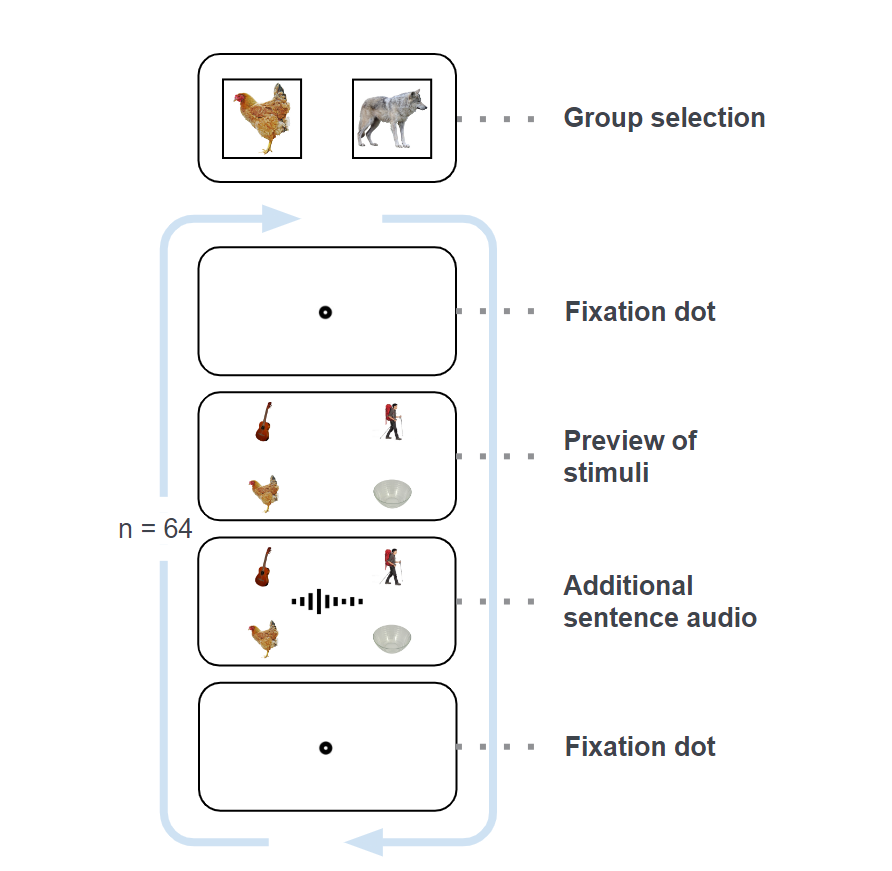
\includegraphics{Images/Fig2_2_1.png}

}

\caption{\label{fig-trials}Experiment procedure with the trial loop.}

\end{figure}%

\section{Materials \& Stimuli}\label{sec-mat-stim}

We have 64 audio stimuli in total with two matching visual stimuli
versions, one consisting of four regular images and the other with four
GIFs. The audio stimuli consisted of different sentences with the same
structure: {[}location/time{]}, {[}person{]} {[}verb{]} {[}object{]},
e.g.: ``At breakfast, the girl ate a croissant.'' The corresponding
visual stimuli consists of four images with only one being closely
related to the sentence. In the case of our example we have one image
being a croissant and the remaining images being random inedible objects
that are not related to breakfast. For the motion stimuli, we just
picked out matching GIFs for the four static images. It was important,
that the gives had the same speed. The exact specifications for static
and motion stimuli as well as the audio stimuli can be found in the
README-File of the experiment.\\
We came up with the 64 different sentences by following the described
structure and created corresponding audios with a free text-to-speech
tool\footnote{https://www.acoust.io/}. For the visual stimuli we re-used
most of the images from the visual world paradigm tutorial by OpenSesame
\footnote{https://osdoc.cogsci.nl/3.3/tutorials/visual-world/} and
looked for additional ones using Google images.

The stimuli creation process turned out to be a cumbersome process with
handling the text-to-speech tool to include breaks and not speak too
fast, finding visual stimuli to go with the audios and making sure that
there is only one matching target sub-stimuli for each sentence. With
our amount of stimuli, it is easy to lose sight of all the different
sub-images. Therefore, to make the stimuli creation process easier, we
used a central excel sheet as documentation where all the sentences and
their corresponding sub-stimuli file names were stated, including which
stimuli version (static or motion) will be shown for each condition
group. In case something changed, we only had to change the central
document and paste its contents to our trial loop in OpenSesame. In
Figure~\ref{fig-stimuli} we provide some stimuli examples:

\begin{figure}

\centering{

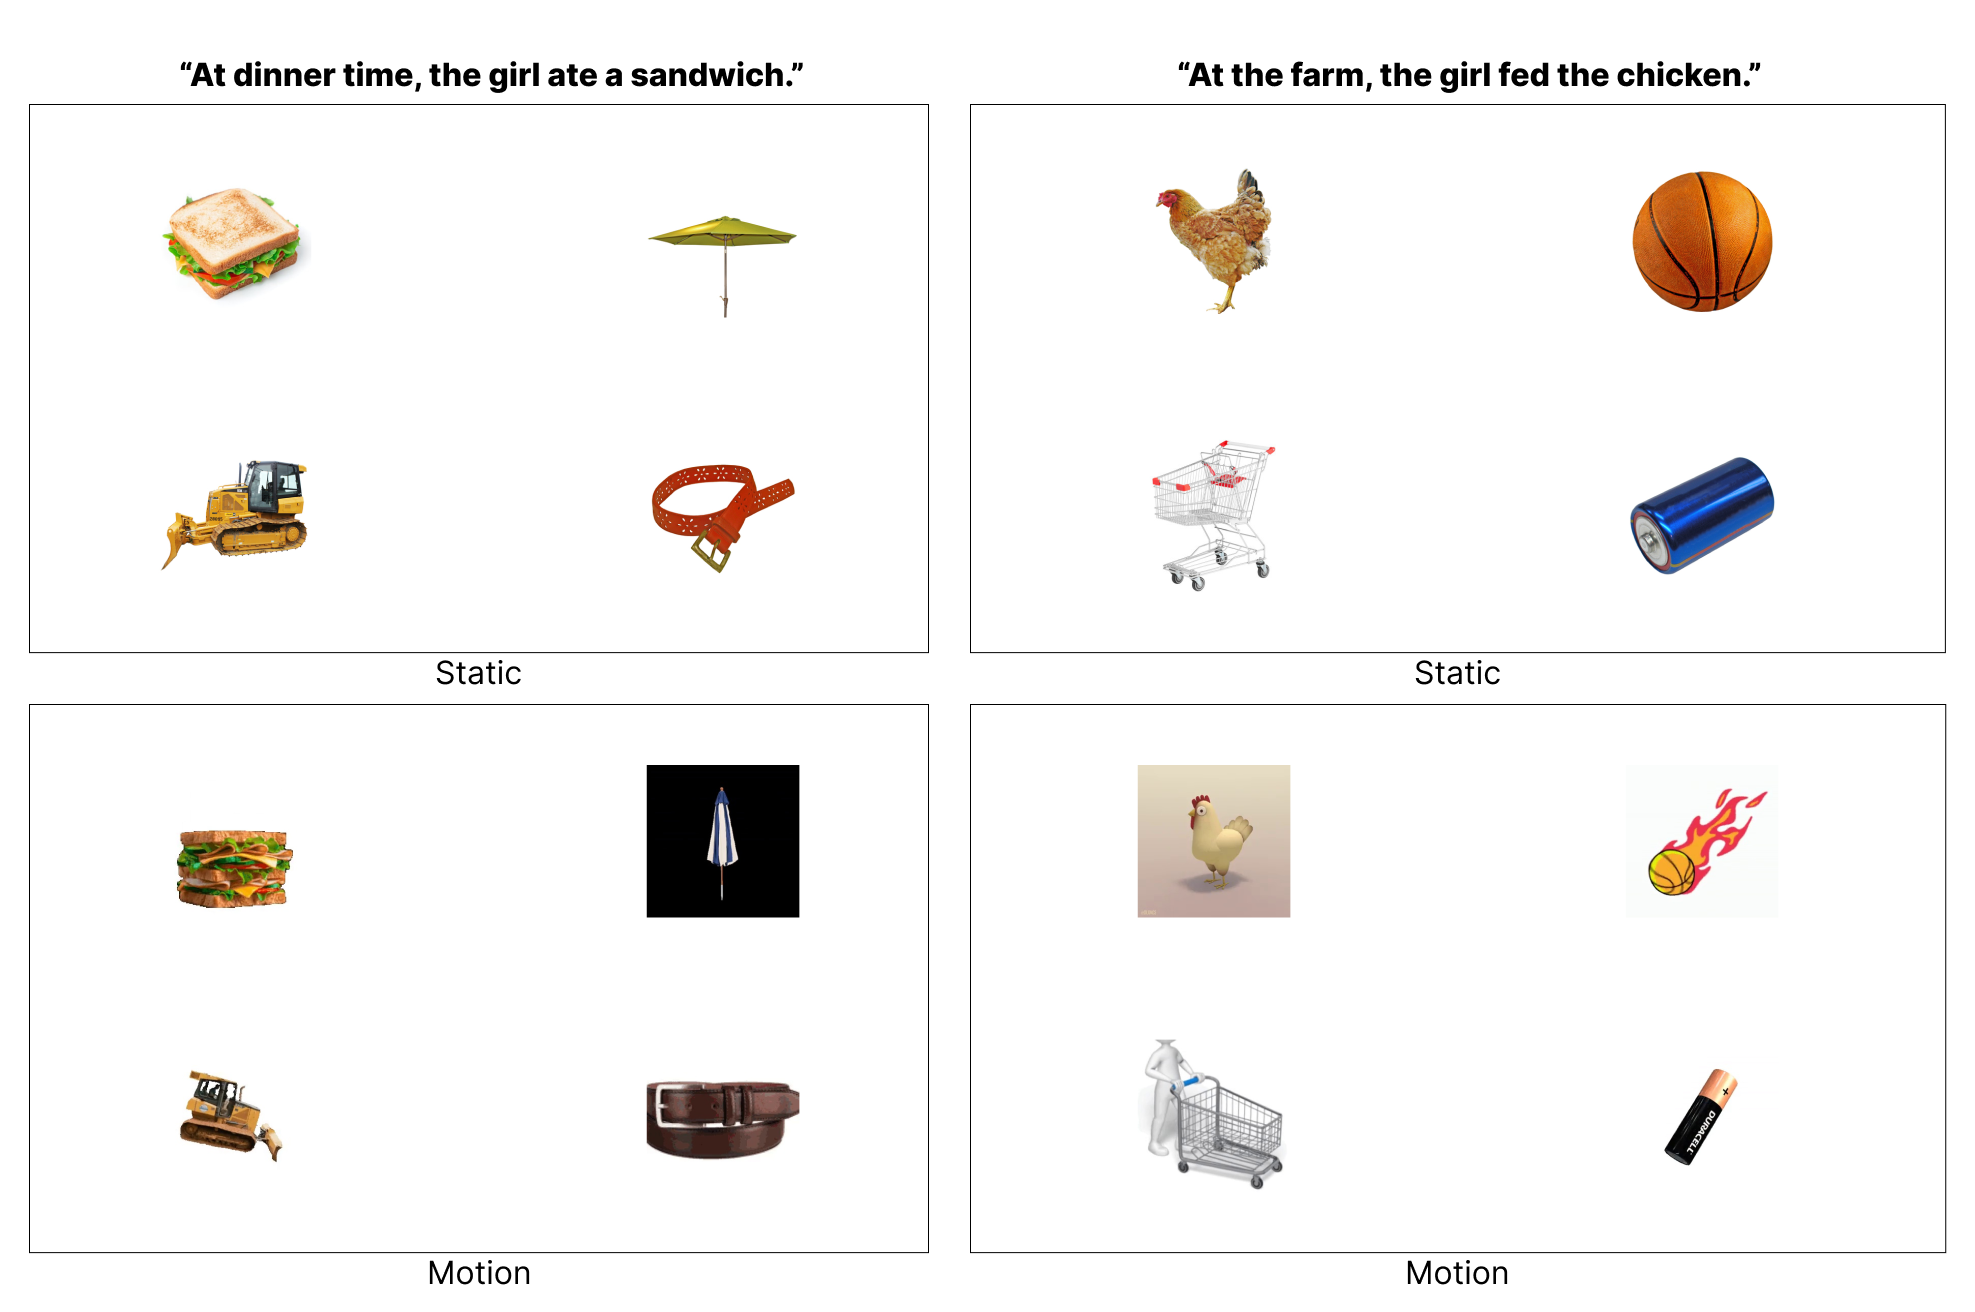
\includegraphics{Images/Fig2_3_1.png}

}

\caption{\label{fig-stimuli}Two example sentences that we used in the
experiment and their respective static and motion visual stimuli.}

\end{figure}%

\section{Study Procedure and Apparatus}\label{sec-stdy-proc}

To test our hypothesis, we needed to invite participants to partake in
our experiment. We recruited participants by asking for volunteers in
our circle of acquaintances and invited the interested people between
mid-July and August. Our target sample size was at least ten
participants to end up with at least five people per condition group.
Once a participant arrived, they were given an information sheet with a
brief description of the experiment, what kind of devices are going to
get used and their corresponding safety risks. Additionally, they were
asked to sign a standard consent form for studies with humans that are
conducted at the university. To counterbalance the number of
participants per condition group, we made them pick a card with a unique
number between 1-10 and depending on whether the ID was an odd number or
not, they got assigned to the corresponding condition group. The
participants were asked to make themselves comfortable on the chair and
adjust it accordingly to their preference, the same goes for the
standard chin rest we used. Both the chair and the chin rest were
disinfected before each participant arrived. To execute the experiment,
we used a standard desktop PC with two displays standing back-to-back in
duplicate view, where one was directed to the participant and the other
was used by the study conductor to start and supervise the experiment.
For tracking, we used the stationary GazePoint GP3 HD eye-tracker in 150
Hz mode. When starting the experiment in OpenSesame, it starts out with
initializing the eye-tracker and calibrating. The calibration process
sometimes took multiple attempts until the results looked precise and
accurate enough. We always told the participants that the calibration
process can require multiple attempts to make sure they dont feel like
they are doing something wrong. After the setup, the experiment itself
lasted around 12 to 15 minutes. The participants had the control to
proceed to the next trial in their own speed and they were informed,
that they can take breaks in-between trials, if needed. Finally, we
asked the participants some basic demographic information and their
previous experiences with eye-tracking. We placed the demographic survey
at the end of the experiment to avoid stereotype threat (see Spencer,
Logel, and Davies (2016)).

\section{Implementation}\label{implementation}

The experiment was conducted using the most recent version of OpenSesame
4.0 Melodramatic Milgram with the PyGame backend. The logic is divided
into three distinct logical units. In the first unit is used to load
custom configuration and preprocess static and motion stimuli. The
config-file was managed with the YAML parser and emitter PyYAML
\footnote{https://pypi.org/project/PyYAML/} and used to customize texts,
their layouts and positions, fixation dots, positions of stimuli as well
as the general timing of the expermient. This way we kept the experiment
flexible for minor changes during the pilot studies or possible future
research. Since it was not possible to display videos or gifs in
OpenSesame, we used the Python library OpenCV \footnote{https://pypi.org/project/opencv-python/}
to extract the frames of each mp4-Videofile and save them into a
separate folder for each stimulus inside a temporary directory. This
directory can be specified in the custom config File, stated above. In
the second unit of the experiment, the built-in calibration of
OpenSesame was used to calibrate the eye-tracker and the group selection
was displayed to the user. The third unit consists of the trial loop.
For each trial, the user is first shown a fixation dot, then the four
substimuli and afterwards the sentence to the pictures is played as
stated in Section~\ref{sec-stdy-proc}. The trial was designed in such a
way that it would only commence once the user had fixated on the central
fixation dot. In order to maintain a consistent framerate for each
motion stimulus, all the images were placed into an infinite loop, with
each sub-stimulus containing an individual frame counter. This counter
was reset to the beginning once it reached the final frame. Any concerns
regarding the performance of the expriment could be cleared after
extensive piloting. Once the designated sentence was played, the
infinite loop was interrupted and the pause screen was displayed. The
logging took place multiple times during the trial loop and finally
logged with the OpenSesame logger. The logging will be discussed in
Section~\ref{sec-logging}.

\chapter{Analysis Methods}\label{sec-analysis}

This chapter shows how data was gathered, preprocessed and analyzed in
order to answer the research question. The analysis was performed in
Python 3.12.4 \footnote{https://www.python.org/downloads/release/python-3124/}
with the use of the libraries Pandas \footnote{https://pypi.org/project/pandas/}
and NumPy \footnote{https://pypi.org/project/numpy/} for data
manipulation and analysis as well as Matplotlib \footnote{https://pypi.org/project/matplotlib/}
and Seaborn \footnote{https://pypi.org/project/seaborn/} for
visualizations. The resulting scripts are Jupyter Notebooks and a Python
script that, depending on the filename, can be run for a single subject
\emph{(e.g.~analysis-subjects.ipynb)} or for all the subjects
\emph{(e.g.~analysis-global.ipynb)}.

\section{Gathering data / logging}\label{sec-logging}

In order to calibrate, record and log the gaze data in OpenSesame, we
used several built-in pygaze elements. For instance, the
\emph{pygaze\_init} element is placed before the trial loop in order to
perform the calibration. Other elements include the
\emph{pygaze\_start\_recording} placed at the beginning of a trial
followed by a logger and a \emph{pygaze\_stop\_recording} at the end of
a trial.

It is essential to record the occurence of specific events during the
experiment, as these will be subject to our subsequent analysis. This is
achieved by custom logging with the logger item in OpenSesame. The
structure of a custom log is always consistent. It comprises of a string
containing all the information from the current row in the stimuli
table. The string is formated in a way that each cell of the row is
logged as key-value pair and divided by a semicolon.

\begin{quote}
VAR TRIAL\_LOG VERB\_CUE=EAT;GROUP=CHICKEN;SENTENCE\_ID=11; SENTENCE=AT
THE FARM, THE GIRL FED THE CHICKEN. ; (\ldots)
\end{quote}

In order to facilitate the differentiation of the current event, a
key-value pair is appended to the log string. Four potential events are
logged within the experiment, as follows:

\begin{itemize}
\tightlist
\item
  Fixation: This event is logged at the beginning of a trial, when the
  participant is presented the fixation dot on the screen.
\item
  Preview: Stimuli are presented.
\item
  Audiostart: The audio with the sentence starts playing.
\item
  Pause: The beginning of the pause, where the user has to look at the
  fixation dot in oder to continue.
\end{itemize}

The subsequent analysis contains two more events which could not be
logged in OpenSesame due to its design. Our solution to this problem
will be presented in the next chapter.

\section{Preprocessing and quality control}\label{sec-pre-quality}

At the beginning, we filtered out the data that was irrelevant for this
research. The dropped columns can be seen in Listing~\ref{lst-del}:

\begin{codelisting}

\caption{\label{lst-del}}

\centering{

\begin{Shaded}
\begin{Highlighting}[]
\CommentTok{\# (...) read data as pandas.DataFrame}

\CommentTok{\# drop irrelevant data}
\NormalTok{data }\OperatorTok{=}\NormalTok{ data.drop([}\StringTok{"TIME\_TICK"}\NormalTok{], axis}\OperatorTok{=}\DecValTok{1}\NormalTok{)}
\NormalTok{data }\OperatorTok{=}\NormalTok{ data.drop([}\StringTok{"FPOGX"}\NormalTok{, }\StringTok{"FPOGY"}\NormalTok{, }\StringTok{"FPOGS"}\NormalTok{, }\StringTok{"FPOGD"}\NormalTok{, }\StringTok{"FPOGID"}\NormalTok{, }\StringTok{"FPOGV"}\NormalTok{], axis}\OperatorTok{=}\DecValTok{1}\NormalTok{) }
\NormalTok{data }\OperatorTok{=}\NormalTok{ data.drop([}\StringTok{"LPOGX"}\NormalTok{, }\StringTok{"LPOGY"}\NormalTok{, }\StringTok{"LPOGV"}\NormalTok{, }\StringTok{"RPOGX"}\NormalTok{, }\StringTok{"RPOGY"}\NormalTok{, }\StringTok{"RPOGV"}\NormalTok{], axis}\OperatorTok{=}\DecValTok{1}\NormalTok{)}
\NormalTok{data }\OperatorTok{=}\NormalTok{ data.drop([}\StringTok{"LPCX"}\NormalTok{, }\StringTok{"LPCY"}\NormalTok{, }\StringTok{"LPD"}\NormalTok{, }\StringTok{"LPS"}\NormalTok{, }\StringTok{"LPV"}\NormalTok{, }\StringTok{"RPCX"}\NormalTok{, }\StringTok{"RPCY"}\NormalTok{, }\StringTok{"RPD"}\NormalTok{, }\StringTok{"RPS"}\NormalTok{, }\StringTok{"RPV"}\NormalTok{], axis}\OperatorTok{=}\DecValTok{1}\NormalTok{)}
\NormalTok{data }\OperatorTok{=}\NormalTok{ data.drop([}\StringTok{"LEYEX"}\NormalTok{, }\StringTok{"LEYEY"}\NormalTok{, }\StringTok{"LEYEZ"}\NormalTok{, }\StringTok{"LPUPILD"}\NormalTok{, }\StringTok{"LPUPILV"}\NormalTok{, }\StringTok{"REYEX"}\NormalTok{, }\StringTok{"REYEY"}\NormalTok{, }\StringTok{"REYEZ"}\NormalTok{, }\StringTok{"RPUPILD"}\NormalTok{, }\StringTok{"RPUPILV"}\NormalTok{], axis}\OperatorTok{=}\DecValTok{1}\NormalTok{)}
\NormalTok{data }\OperatorTok{=}\NormalTok{ data.drop([}\StringTok{"CX"}\NormalTok{, }\StringTok{"CY"}\NormalTok{, }\StringTok{"CS"}\NormalTok{], axis}\OperatorTok{=}\DecValTok{1}\NormalTok{)}
\end{Highlighting}
\end{Shaded}

}

\end{codelisting}%

The resulting Dataframe looks like this:

\begin{longtable}[]{@{}ccccc@{}}
\caption{Filtered raw gaze data of a
participant}\label{tbl-a}\tabularnewline
\toprule\noalign{}
TIME & BPOGX & BPOGY & BPOGV & USER \\
\midrule\noalign{}
\endfirsthead
\toprule\noalign{}
TIME & BPOGX & BPOGY & BPOGV & USER \\
\midrule\noalign{}
\endhead
\bottomrule\noalign{}
\endlastfoot
204.69383 & 0.33433 & 0.57871 & 1 & START\_TRIAL 0 \\
\end{longtable}

Resulting data and its interpretation can be found in the GazePoint API
documentation \footnote{https://www.gazept.com/dl/Gazepoint\_API\_v2.0.pdf}
and forms the basis for the analysis.

At the beginning several sanity checks were performed in order to
evaluate the quality of the collected data. The first one being the
examination on recorded logs. Therefor the occurencies of all existing
logs in the USER column were counted. Since the experiment has 64 trials
there should be 64 hits for each log message except the
\emph{TRIAL\_WARNING} that is only logged when the subject does not
fixate on the fixation dot during a pause for more than 15 seconds.
Afterwards the results are plotted in a barplot (see
Figure~\ref{fig-barplt-evts} and Listing~\ref{lst-barplot-events}).

\begin{figure}

\centering{

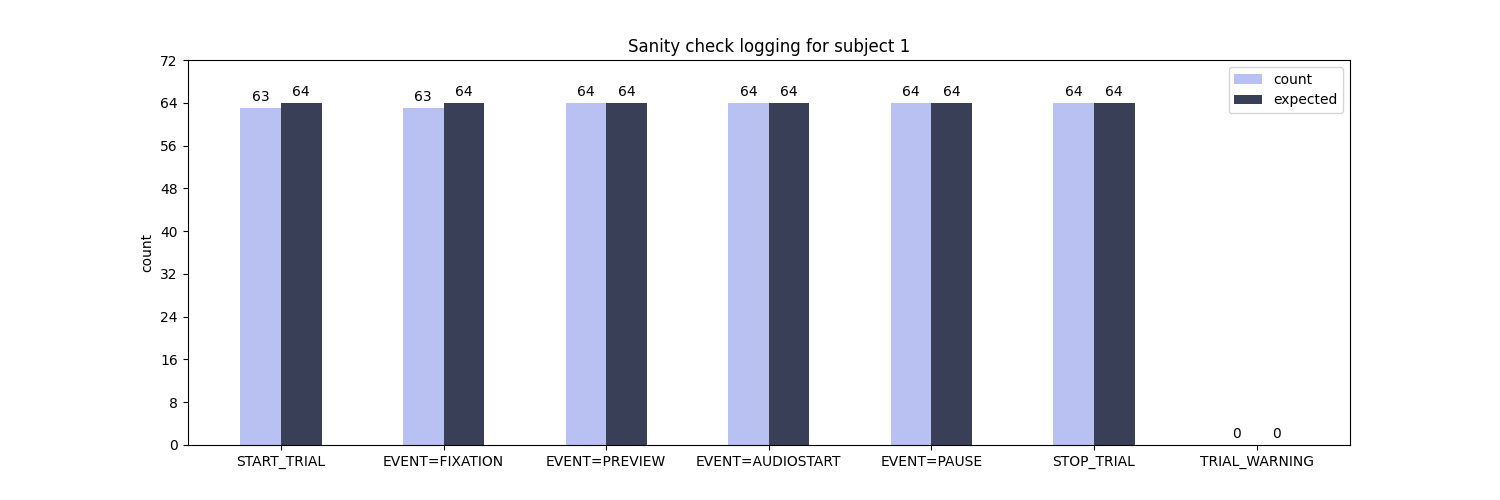
\includegraphics{Images/Fig3_2_0.png}

}

\caption{\label{fig-barplt-evts}Counted vs.~expected logs for an example
subject}

\end{figure}%

\begin{codelisting}

\caption{\label{lst-barplot-events}}

\centering{

\begin{Shaded}
\begin{Highlighting}[]
\CommentTok{\# finds the occurencies of "word" in data}
\KeywordTok{def}\NormalTok{ find\_occur(data, word):}
\NormalTok{    all\_text }\OperatorTok{=} \StringTok{" "}\NormalTok{.join(data[}\StringTok{"USER"}\NormalTok{].astype(}\BuiltInTok{str}\NormalTok{).values.flatten())}
\NormalTok{    total\_count }\OperatorTok{=}\NormalTok{ all\_text.count(word)}
    \ControlFlowTok{return}\NormalTok{ total\_count}

\CommentTok{\# (...)}

\CommentTok{\# index}
\NormalTok{log\_index }\OperatorTok{=}\NormalTok{ [}\StringTok{"START\_TRIAL"}\NormalTok{, }\StringTok{"EVENT=FIXATION"}\NormalTok{, }\StringTok{"EVENT=PREVIEW"}\NormalTok{, }\StringTok{"EVENT=AUDIOSTART"}\NormalTok{, }\StringTok{"EVENT=PAUSE"}\NormalTok{, }\StringTok{"STOP\_TRIAL"}\NormalTok{, }\StringTok{"TRIAL\_WARNING"}\NormalTok{]}
\NormalTok{ind }\OperatorTok{=}\NormalTok{ np.arange(}\BuiltInTok{len}\NormalTok{(log\_index))}

\CommentTok{\# count occurencies of each word}
\NormalTok{count }\OperatorTok{=}\NormalTok{ []}
\ControlFlowTok{for}\NormalTok{ log }\KeywordTok{in}\NormalTok{ log\_index:}
\NormalTok{    count.append(find\_occur(data, log))}

\CommentTok{\# load data into dataframe}
\NormalTok{logs }\OperatorTok{=}\NormalTok{ pd.DataFrame(\{}\StringTok{"count"}\NormalTok{: count, }\StringTok{"expected"}\NormalTok{: expected\_logs\}, index}\OperatorTok{=}\NormalTok{log\_index)}

\CommentTok{\# (...) plot data}
\end{Highlighting}
\end{Shaded}

}

\end{codelisting}%

By plotting a histogram of the time delta between samples, we found out,
that it is not consistent. Therefor we interpolated the values of BPOGX,
BPOGY, and BPOGV with the scipy \footnote{https://pypi.org/project/scipy/}
linear (one dimensional) interpolator (see
Listing~\ref{lst-interp-code}). The time was reorganized in a way that
it matches the sampling rate. Since the eye-tracker has a sampling rate
of 150 Hz, the total time of the experiment in seconds was multiplyed by
150 to figure out the amount of bins for the interpolation function. The
respective values for BPOGX, BPOGY and BPOGV at the location of each bin
determined the interpolated value. In order to obtain a valid BPOGV, its
value after interpolation was rounded to an integer value.

\begin{codelisting}

\caption{\label{lst-interp-code}}

\centering{

\begin{Shaded}
\begin{Highlighting}[]
\CommentTok{\# (...)}
\CommentTok{\# interpolate BPOGX and BPOGY}
\NormalTok{interp\_func\_x }\OperatorTok{=}\NormalTok{ interp1d(data[}\StringTok{"TIME"}\NormalTok{], data[}\StringTok{"BPOGX"}\NormalTok{], kind}\OperatorTok{=}\StringTok{"linear"}\NormalTok{, fill\_value}\OperatorTok{=}\StringTok{"interpolate"}\NormalTok{)}
\NormalTok{interp\_func\_y }\OperatorTok{=}\NormalTok{ interp1d(data[}\StringTok{"TIME"}\NormalTok{], data[}\StringTok{"BPOGY"}\NormalTok{], kind}\OperatorTok{=}\StringTok{"linear"}\NormalTok{, fill\_value}\OperatorTok{=}\StringTok{"interpolate"}\NormalTok{)}
\NormalTok{interp\_func\_v }\OperatorTok{=}\NormalTok{ interp1d(data[}\StringTok{"TIME"}\NormalTok{], data[}\StringTok{"BPOGV"}\NormalTok{], kind}\OperatorTok{=}\StringTok{"linear"}\NormalTok{, fill\_value}\OperatorTok{=}\StringTok{"interpolate"}\NormalTok{)}

\CommentTok{\# generate new evenly spaced time points}
\NormalTok{t\_delta }\OperatorTok{=}\NormalTok{ data[}\StringTok{"TIME"}\NormalTok{].}\BuiltInTok{max}\NormalTok{() }\OperatorTok{{-}}\NormalTok{ data[}\StringTok{"TIME"}\NormalTok{].}\BuiltInTok{min}\NormalTok{() }
\NormalTok{lin\_num }\OperatorTok{=}\NormalTok{ (t\_delta }\OperatorTok{*}\NormalTok{ sample\_rate).}\BuiltInTok{round}\NormalTok{(}\DecValTok{0}\NormalTok{).astype(}\BuiltInTok{int}\NormalTok{)}

\NormalTok{new\_time }\OperatorTok{=}\NormalTok{ np.linspace(data[}\StringTok{"TIME"}\NormalTok{].}\BuiltInTok{min}\NormalTok{(), data[}\StringTok{"TIME"}\NormalTok{].}\BuiltInTok{max}\NormalTok{(), num}\OperatorTok{=}\NormalTok{lin\_num)}

\CommentTok{\# get interpolated values with new time}
\NormalTok{new\_bpogx }\OperatorTok{=}\NormalTok{ interp\_func\_x(new\_time)}
\NormalTok{new\_bpogy }\OperatorTok{=}\NormalTok{ interp\_func\_y(new\_time)}
\NormalTok{new\_bpogv }\OperatorTok{=}\NormalTok{ interp\_func\_v(new\_time)}

\CommentTok{\# overwrite original dataframe and round like original data}
\NormalTok{data }\OperatorTok{=}\NormalTok{ pd.DataFrame(\{\})}
\NormalTok{data[}\StringTok{"TIME"}\NormalTok{] }\OperatorTok{=}\NormalTok{ new\_time}
\NormalTok{data[}\StringTok{"BPOGX"}\NormalTok{] }\OperatorTok{=}\NormalTok{ new\_bpogx.astype(}\BuiltInTok{float}\NormalTok{)}
\NormalTok{data[}\StringTok{"BPOGY"}\NormalTok{] }\OperatorTok{=}\NormalTok{ new\_bpogy.astype(}\BuiltInTok{float}\NormalTok{)}
\NormalTok{data[}\StringTok{"BPOGV"}\NormalTok{] }\OperatorTok{=}\NormalTok{ new\_bpogv.}\BuiltInTok{round}\NormalTok{(}\DecValTok{0}\NormalTok{).astype(}\BuiltInTok{int}\NormalTok{)}

\KeywordTok{def}\NormalTok{ find\_nearest\_index(array, value):}
\NormalTok{    idx }\OperatorTok{=}\NormalTok{ (np.}\BuiltInTok{abs}\NormalTok{(array }\OperatorTok{{-}}\NormalTok{ value)).argmin()}
    \ControlFlowTok{return}\NormalTok{ idx}

\CommentTok{\# map user events back to correct time}
\ControlFlowTok{for}\NormalTok{ index, row }\KeywordTok{in}\NormalTok{ before\_interpol\_data.iterrows():}
    \ControlFlowTok{if}\NormalTok{ pd.notna(row[}\StringTok{"USER"}\NormalTok{]):  }\CommentTok{\# Check if USER event is present}
\NormalTok{        nearest\_index }\OperatorTok{=}\NormalTok{ find\_nearest\_index(new\_time, row[}\StringTok{"TIME"}\NormalTok{])}
        \CommentTok{\# Add or append the event to the USER column}
\NormalTok{        data.at[nearest\_index, }\StringTok{"USER"}\NormalTok{] }\OperatorTok{=}\NormalTok{ row[}\StringTok{"USER"}\NormalTok{]}
\end{Highlighting}
\end{Shaded}

}

\end{codelisting}%

Figure~\ref{fig-interpolation} shows an example function before and
after interpolation:

\begin{figure}

\centering{

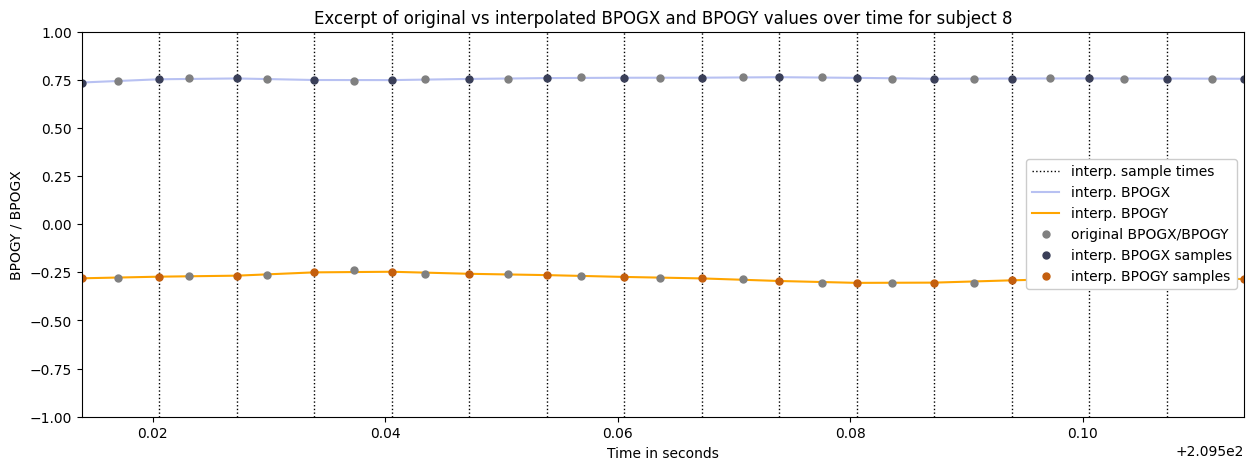
\includegraphics{Images/Fig3_2_1.png}

}

\caption{\label{fig-interpolation}Interpolation}

\end{figure}%

In the next step the custom logs were decoded. In this process, the rows
of the dataframe containing a \emph{TRIAL\_LOG} in the \emph{USER}
column were filtered and the logsting was decoded. Therefore all
key-value pairs were split and for each key a new column was created.
The respective value was placed in the current row of the key-column.
Afterwards, the \emph{USER} column was dropped. A row that contained a
log looks for example like that:

\begin{longtable}[]{@{}
  >{\centering\arraybackslash}p{(\columnwidth - 20\tabcolsep) * \real{0.1667}}
  >{\centering\arraybackslash}p{(\columnwidth - 20\tabcolsep) * \real{0.1500}}
  >{\centering\arraybackslash}p{(\columnwidth - 20\tabcolsep) * \real{0.1667}}
  >{\centering\arraybackslash}p{(\columnwidth - 20\tabcolsep) * \real{0.0500}}
  >{\centering\arraybackslash}p{(\columnwidth - 20\tabcolsep) * \real{0.0667}}
  >{\centering\arraybackslash}p{(\columnwidth - 20\tabcolsep) * \real{0.0667}}
  >{\centering\arraybackslash}p{(\columnwidth - 20\tabcolsep) * \real{0.0667}}
  >{\centering\arraybackslash}p{(\columnwidth - 20\tabcolsep) * \real{0.0667}}
  >{\centering\arraybackslash}p{(\columnwidth - 20\tabcolsep) * \real{0.0667}}
  >{\centering\arraybackslash}p{(\columnwidth - 20\tabcolsep) * \real{0.0667}}
  >{\centering\arraybackslash}p{(\columnwidth - 20\tabcolsep) * \real{0.0667}}@{}}
\caption{Decoded custom logs in dataframe with gaze
data}\label{tbl-b}\tabularnewline
\toprule\noalign{}
\begin{minipage}[b]{\linewidth}\centering
TIME
\end{minipage} & \begin{minipage}[b]{\linewidth}\centering
(\ldots)
\end{minipage} & \begin{minipage}[b]{\linewidth}\centering
BPOGV
\end{minipage} & \begin{minipage}[b]{\linewidth}\centering
SUBJECT
\end{minipage} & \begin{minipage}[b]{\linewidth}\centering
EVENT
\end{minipage} & \begin{minipage}[b]{\linewidth}\centering
TRIAL
\end{minipage} & \begin{minipage}[b]{\linewidth}\centering
GROUP
\end{minipage} & \begin{minipage}[b]{\linewidth}\centering
(\ldots)
\end{minipage} & \begin{minipage}[b]{\linewidth}\centering
VERB\_CUE
\end{minipage} & \begin{minipage}[b]{\linewidth}\centering
TARGET\_CUE\_TIMING
\end{minipage} & \begin{minipage}[b]{\linewidth}\centering
\end{minipage} \\
\midrule\noalign{}
\endfirsthead
\toprule\noalign{}
\begin{minipage}[b]{\linewidth}\centering
TIME
\end{minipage} & \begin{minipage}[b]{\linewidth}\centering
(\ldots)
\end{minipage} & \begin{minipage}[b]{\linewidth}\centering
BPOGV
\end{minipage} & \begin{minipage}[b]{\linewidth}\centering
SUBJECT
\end{minipage} & \begin{minipage}[b]{\linewidth}\centering
EVENT
\end{minipage} & \begin{minipage}[b]{\linewidth}\centering
TRIAL
\end{minipage} & \begin{minipage}[b]{\linewidth}\centering
GROUP
\end{minipage} & \begin{minipage}[b]{\linewidth}\centering
(\ldots)
\end{minipage} & \begin{minipage}[b]{\linewidth}\centering
VERB\_CUE
\end{minipage} & \begin{minipage}[b]{\linewidth}\centering
TARGET\_CUE\_TIMING
\end{minipage} & \begin{minipage}[b]{\linewidth}\centering
\end{minipage} \\
\midrule\noalign{}
\endhead
\bottomrule\noalign{}
\endlastfoot
1487.3\ldots{} & (\ldots) & 1 & 3 & FIXATION & 0 & WOLF & (\ldots) &
SERVED & 2115 & \\
\end{longtable}

\begin{codelisting}

\caption{\label{lst-cust-log-dec}}

\centering{

\begin{Shaded}
\begin{Highlighting}[]
\ControlFlowTok{for}\NormalTok{ index, row }\KeywordTok{in}\NormalTok{ data.iterrows():}
    
    \CommentTok{\# add subject to every row}
\NormalTok{    data.at[index, }\StringTok{"SUBJECT"}\NormalTok{] }\OperatorTok{=}\NormalTok{ subject\_no}

    \CommentTok{\# get loggin row of opengaze data}
\NormalTok{    inp }\OperatorTok{=} \BuiltInTok{str}\NormalTok{(row[}\StringTok{"USER"}\NormalTok{])}
    
    \ControlFlowTok{if}\NormalTok{ inp.find(}\StringTok{"TRIAL\_LOG"}\NormalTok{) }\OperatorTok{!=} \OperatorTok{{-}}\DecValTok{1}\NormalTok{:}
        
\NormalTok{        cleaned\_inp }\OperatorTok{=}\NormalTok{ inp.split(}\StringTok{"VAR TRIAL\_LOG "}\NormalTok{, maxsplit}\OperatorTok{=}\DecValTok{2}\NormalTok{)[}\DecValTok{1}\NormalTok{]}
\NormalTok{        kv\_inp }\OperatorTok{=}\NormalTok{ cleaned\_inp.split(}\StringTok{";"}\NormalTok{)}

        \CommentTok{\# decode key/value{-}pairs and copy them to column (key) and value (cell)}
        \ControlFlowTok{for}\NormalTok{ elem }\KeywordTok{in}\NormalTok{ kv\_inp:}

\NormalTok{            key, val }\OperatorTok{=}\NormalTok{ elem.split(}\StringTok{"="}\NormalTok{, maxsplit}\OperatorTok{=}\DecValTok{1}\NormalTok{)}

\NormalTok{            data.at[index, key] }\OperatorTok{=}\NormalTok{ val}
    
    \CommentTok{\# other custom logs}
    \ControlFlowTok{elif}\NormalTok{ inp.find(}\StringTok{"TRIAL\_WARNING"}\NormalTok{) }\OperatorTok{!=} \OperatorTok{{-}}\DecValTok{1}\NormalTok{:}
        
\NormalTok{        data.at[index, }\StringTok{"EVENT"}\NormalTok{] }\OperatorTok{=} \StringTok{"WARNING"}
        
    \ControlFlowTok{elif}\NormalTok{ inp.find(}\StringTok{"START\_TRIAL"}\NormalTok{) }\OperatorTok{!=} \OperatorTok{{-}}\DecValTok{1}\NormalTok{:}
        
\NormalTok{        data.at[index, }\StringTok{"EVENT"}\NormalTok{] }\OperatorTok{=} \StringTok{"START\_TRIAL"}
\NormalTok{        data.at[index, }\StringTok{"TRIAL"}\NormalTok{] }\OperatorTok{=} \BuiltInTok{int}\NormalTok{(inp[}\DecValTok{11}\NormalTok{:].replace(}\StringTok{" "}\NormalTok{, }\StringTok{""}\NormalTok{))}
    
    \ControlFlowTok{elif}\NormalTok{ inp.find(}\StringTok{"STOP\_TRIAL"}\NormalTok{) }\OperatorTok{!=} \OperatorTok{{-}}\DecValTok{1}\NormalTok{:}
        
\NormalTok{        data.at[index, }\StringTok{"EVENT"}\NormalTok{] }\OperatorTok{=} \StringTok{"STOP\_TRIAL"}
\NormalTok{        data.at[index, }\StringTok{"TRIAL"}\NormalTok{] }\OperatorTok{=} \BuiltInTok{int}\NormalTok{(inp[}\DecValTok{11}\NormalTok{:].replace(}\StringTok{" "}\NormalTok{, }\StringTok{""}\NormalTok{))}

\CommentTok{\# drop original log column}
\NormalTok{data.drop(columns}\OperatorTok{=}\NormalTok{[}\StringTok{"USER"}\NormalTok{], inplace}\OperatorTok{=}\VariableTok{True}\NormalTok{)}
\end{Highlighting}
\end{Shaded}

}

\end{codelisting}%

As mentioned in Section~\ref{sec-logging}, two events can not be logged
due to the design of OpenSesame. These events are \emph{VERBONSET} and
\emph{TARGETONSET}. \emph{VERBONSET} refers to the time, when the
sentence is played to the subject and the verb of the sentence is said.
\emph{TARGETONSET} is the exact timing where the target word of the
sentence is spoken. The in Section~\ref{sec-mat-stim} introduced
stimuli-table \footnote{Can be found in the project folder under
  \textasciitilde/stimuli/0-stimuli-table.xlsx} also contains for each
sentence the audio and the time that has passed until the verb and the
target word is said. We consider this two time intervals as deltas.
Afterwards we took the time were the \emph{AUDIOSTART} event happened
and added each time interval to the \emph{AUDIOSTART}-time. The
resulting times are the values \emph{VERB- and TARGETONSET}.
Figure~\ref{fig-verbtargetonset} illustrates this process.

\begin{figure}

\centering{

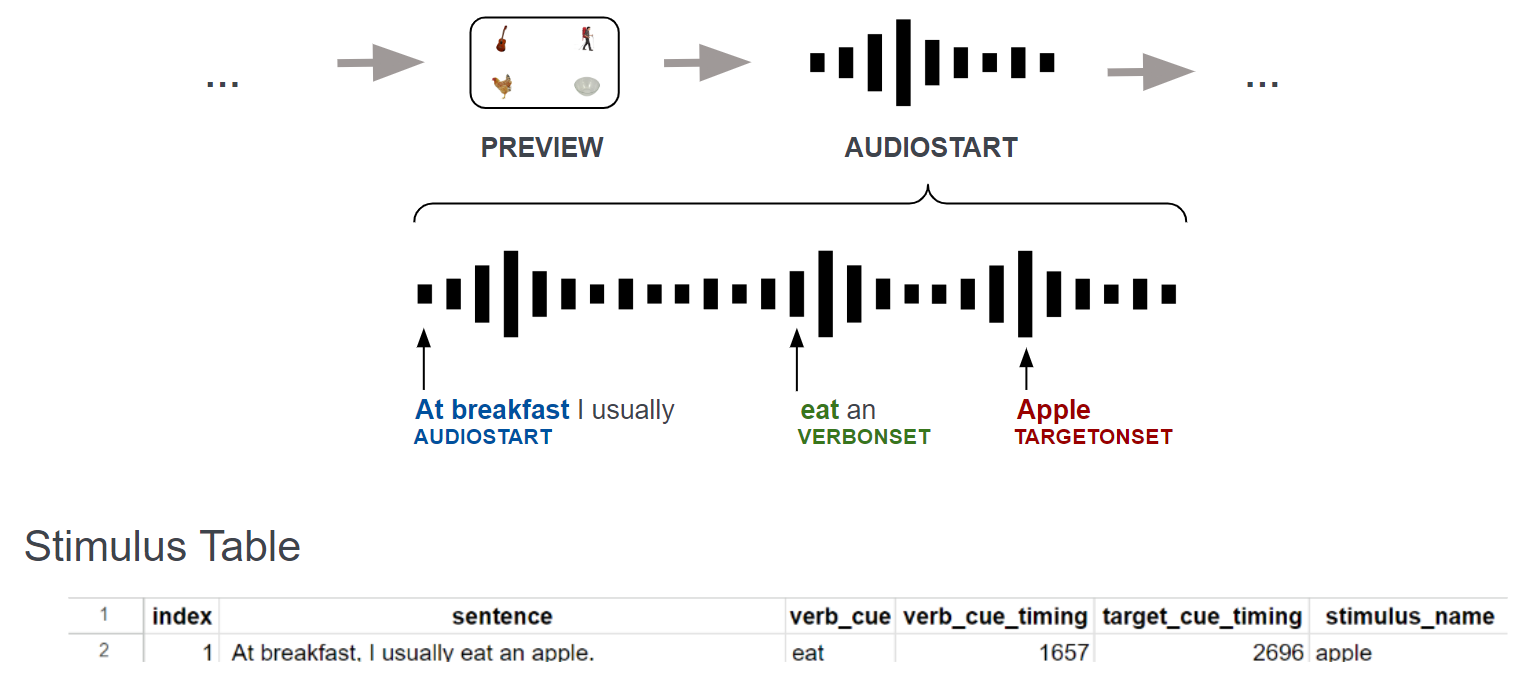
\includegraphics{Images/Fig3_2_2.png}

}

\caption{\label{fig-verbtargetonset}Connection between event cues
AUDIOSTART, VERB- and TARGETONSET}

\end{figure}%

\begin{codelisting}

\caption{\label{lst-cust-calc-verb-taget-onset}}

\centering{

\begin{Shaded}
\begin{Highlighting}[]
\CommentTok{\# extend logs with the corresponding events}
\NormalTok{audio\_start\_data }\OperatorTok{=}\NormalTok{ data.query(}\StringTok{"EVENT==\textquotesingle{}AUDIOSTART\textquotesingle{}"}\NormalTok{)}

\ControlFlowTok{for}\NormalTok{ index, row }\KeywordTok{in}\NormalTok{ audio\_start\_data.iterrows():}
    
\NormalTok{    sample\_time }\OperatorTok{=} \BuiltInTok{float}\NormalTok{(row[}\StringTok{"TIME"}\NormalTok{])}
    
\NormalTok{    delta\_verb\_onset }\OperatorTok{=} \BuiltInTok{float}\NormalTok{(row[}\StringTok{"VERB\_CUE\_TIMING"}\NormalTok{])}\OperatorTok{/}\DecValTok{1000}
\NormalTok{    delta\_target\_onset }\OperatorTok{=} \BuiltInTok{float}\NormalTok{(row[}\StringTok{"TARGET\_CUE\_TIMING"}\NormalTok{])}\OperatorTok{/}\DecValTok{1000}
    
\NormalTok{    time\_verb\_onset }\OperatorTok{=}\NormalTok{ sample\_time }\OperatorTok{+}\NormalTok{ delta\_verb\_onset}
\NormalTok{    time\_target\_onset }\OperatorTok{=}\NormalTok{ sample\_time }\OperatorTok{+}\NormalTok{ delta\_target\_onset}
    
\NormalTok{    first\_sample\_verb }\OperatorTok{=}\NormalTok{ data[data[}\StringTok{"TIME"}\NormalTok{] }\OperatorTok{\textgreater{}=}\NormalTok{ time\_verb\_onset].iloc[}\DecValTok{0}\NormalTok{].name}
\NormalTok{    first\_sample\_target }\OperatorTok{=}\NormalTok{ data[data[}\StringTok{"TIME"}\NormalTok{] }\OperatorTok{\textgreater{}=}\NormalTok{ time\_target\_onset].iloc[}\DecValTok{0}\NormalTok{].name}
    
    \ControlFlowTok{for}\NormalTok{ field }\KeywordTok{in}\NormalTok{ fields\_to\_copy:}
\NormalTok{        data.at[first\_sample\_verb, field] }\OperatorTok{=}\NormalTok{ row[field]}
\NormalTok{        data.at[first\_sample\_target, field] }\OperatorTok{=}\NormalTok{ row[field]}
    
    \CommentTok{\# Set the EVENT to "VERBONSET"}
\NormalTok{    data.at[first\_sample\_verb, }\StringTok{"EVENT"}\NormalTok{] }\OperatorTok{=} \StringTok{"VERBONSET"}
\NormalTok{    data.at[first\_sample\_target, }\StringTok{"EVENT"}\NormalTok{] }\OperatorTok{=} \StringTok{"TARGETONSET"}
\end{Highlighting}
\end{Shaded}

}

\end{codelisting}%

Finally the format of rows that contained mixed characters was unified
and the resulting dataframe as exported into a csv file under the
\emph{\textasciitilde/data/preprocessed/} directory.

\begin{codelisting}

\caption{\label{lst-format-check}}

\centering{

\begin{Shaded}
\begin{Highlighting}[]
\NormalTok{data[}\StringTok{"SUBJECT"}\NormalTok{] }\OperatorTok{=}\NormalTok{ data[}\StringTok{"SUBJECT"}\NormalTok{].fillna(}\DecValTok{0}\NormalTok{).astype(}\BuiltInTok{int}\NormalTok{)}
\NormalTok{data[}\StringTok{"TRIAL"}\NormalTok{] }\OperatorTok{=}\NormalTok{ data[}\StringTok{"TRIAL"}\NormalTok{].fillna(}\DecValTok{0}\NormalTok{).astype(}\BuiltInTok{int}\NormalTok{)}
\NormalTok{data[}\StringTok{"SENTENCE\_ID"}\NormalTok{] }\OperatorTok{=}\NormalTok{ data[}\StringTok{"SENTENCE\_ID"}\NormalTok{].fillna(}\DecValTok{0}\NormalTok{).astype(}\BuiltInTok{int}\NormalTok{)}
\end{Highlighting}
\end{Shaded}

}

\end{codelisting}%

This concludes the Section~\ref{sec-pre-quality} chapter. The full
script for the preprocessing is enclosed in the form of a Jupyter
notebook and can be found in the project path
\emph{\textasciitilde/scripts/preprocess-subject.ipynb}.

\section{Measurements, Metrics and
Visualisations}\label{measurements-metrics-and-visualisations}

To verify the correctness, consistency and accuracy of the data
collected, especially during the piloting trials, several visualizations
were employed. The first one being visualization of the BPOGX and BPOGY
coordinates was generated (see Fig. Figure~\ref{fig-bpogxy}). This plot
illustrated the raw gaze points captured by the eye tracker across the
screen.

\begin{figure}

\centering{

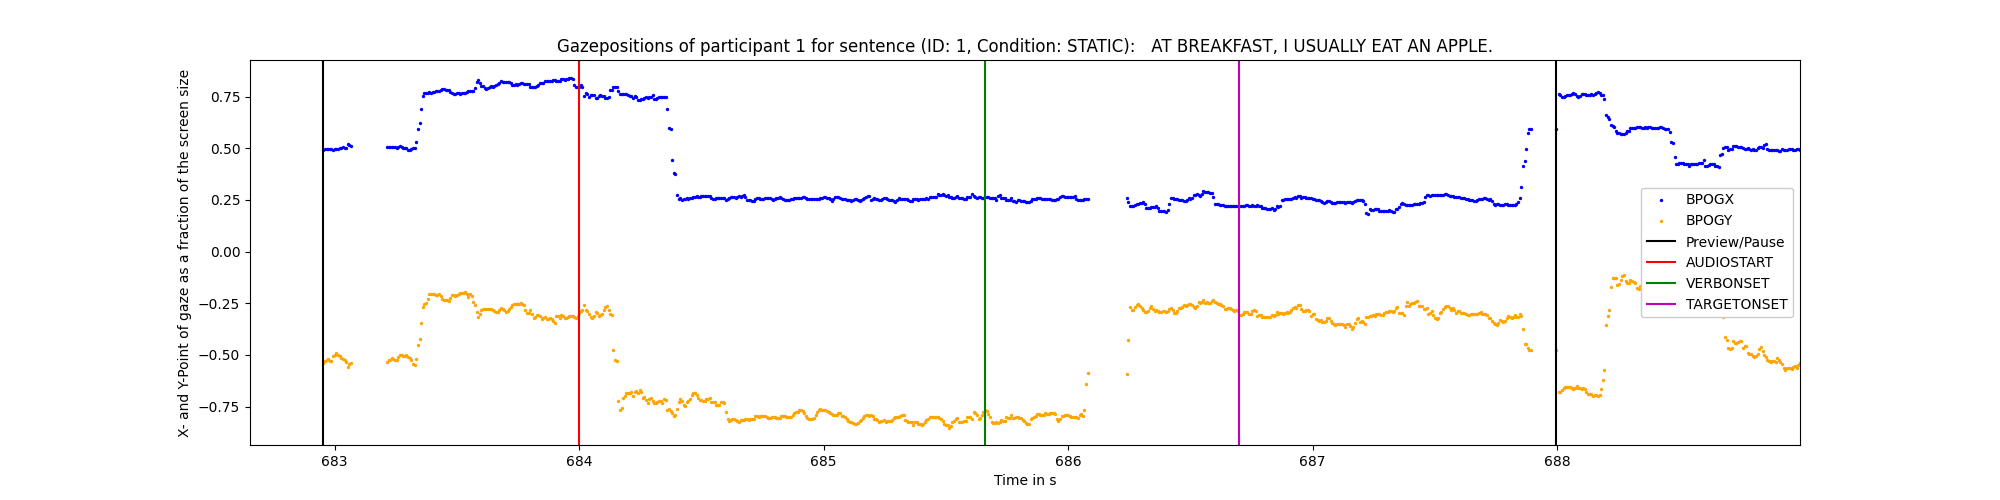
\includegraphics{Images/Fig4_4_0.png}

}

\caption{\label{fig-bpogxy}Example of best point of gaze for a sentence}

\end{figure}%

The scanpath visualization (see Figure~\ref{fig-scanpath}) was used to
trace the path that a subjects eye-movements took to ensure alignment
with the expected gaze patterns. The heatmaps (see
Figure~\ref{fig-heatmap}) allowed quick verification of attention
directed towards the defined areas of interest (AOI).

\begin{figure}

\centering{

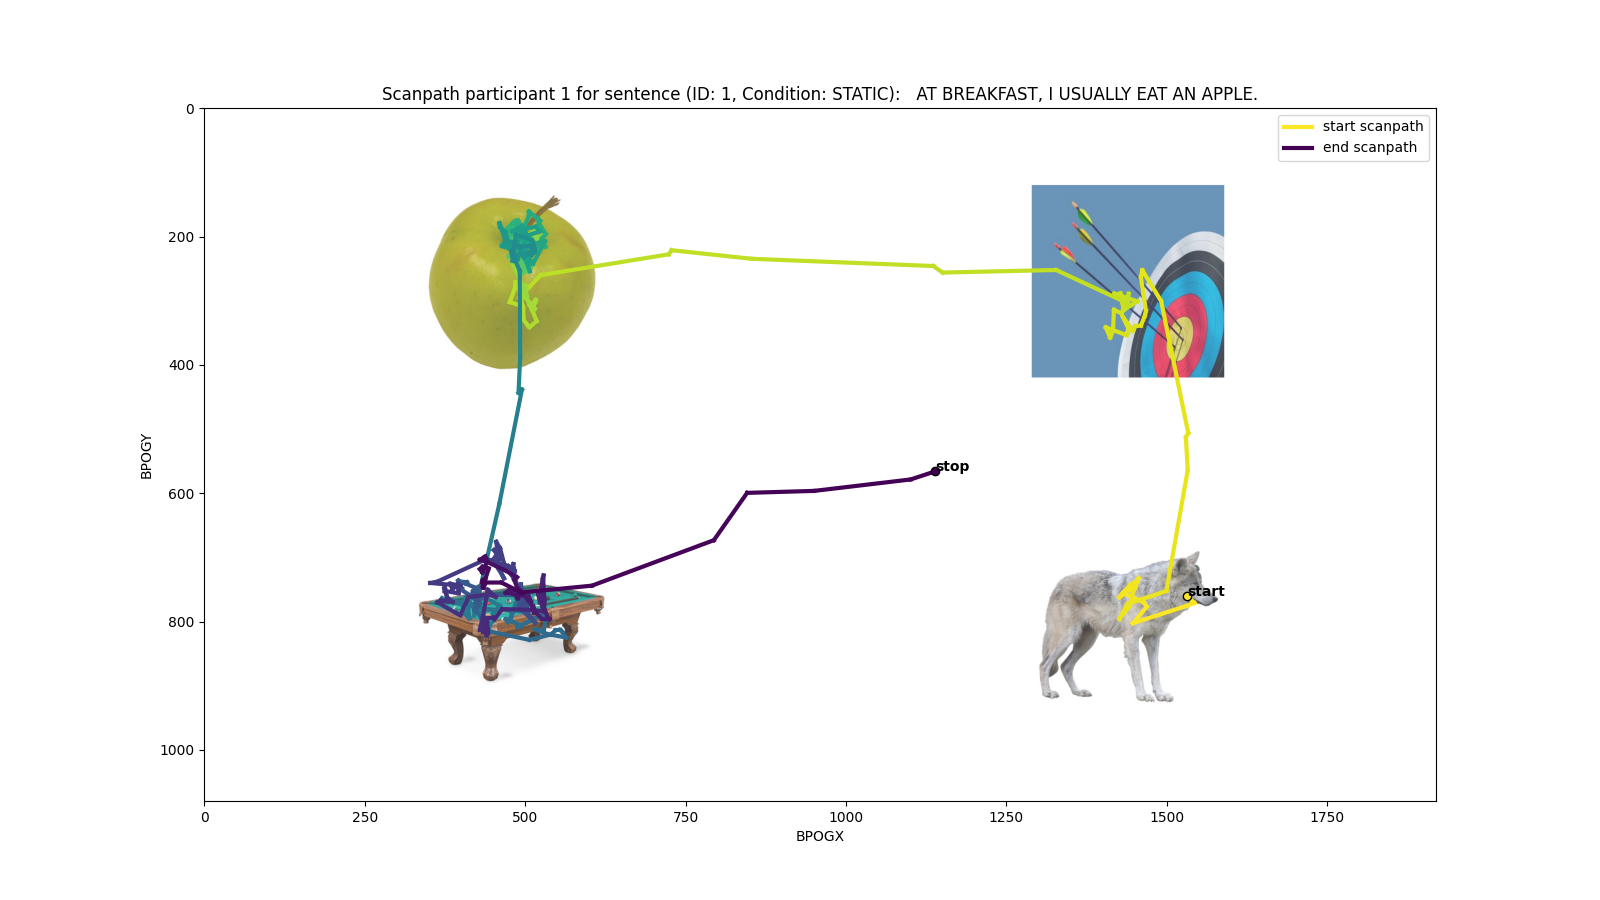
\includegraphics{Images/Fig4_4_1.png}

}

\caption{\label{fig-scanpath}Example scanpath for a sentence}

\end{figure}%

\begin{figure}

\centering{

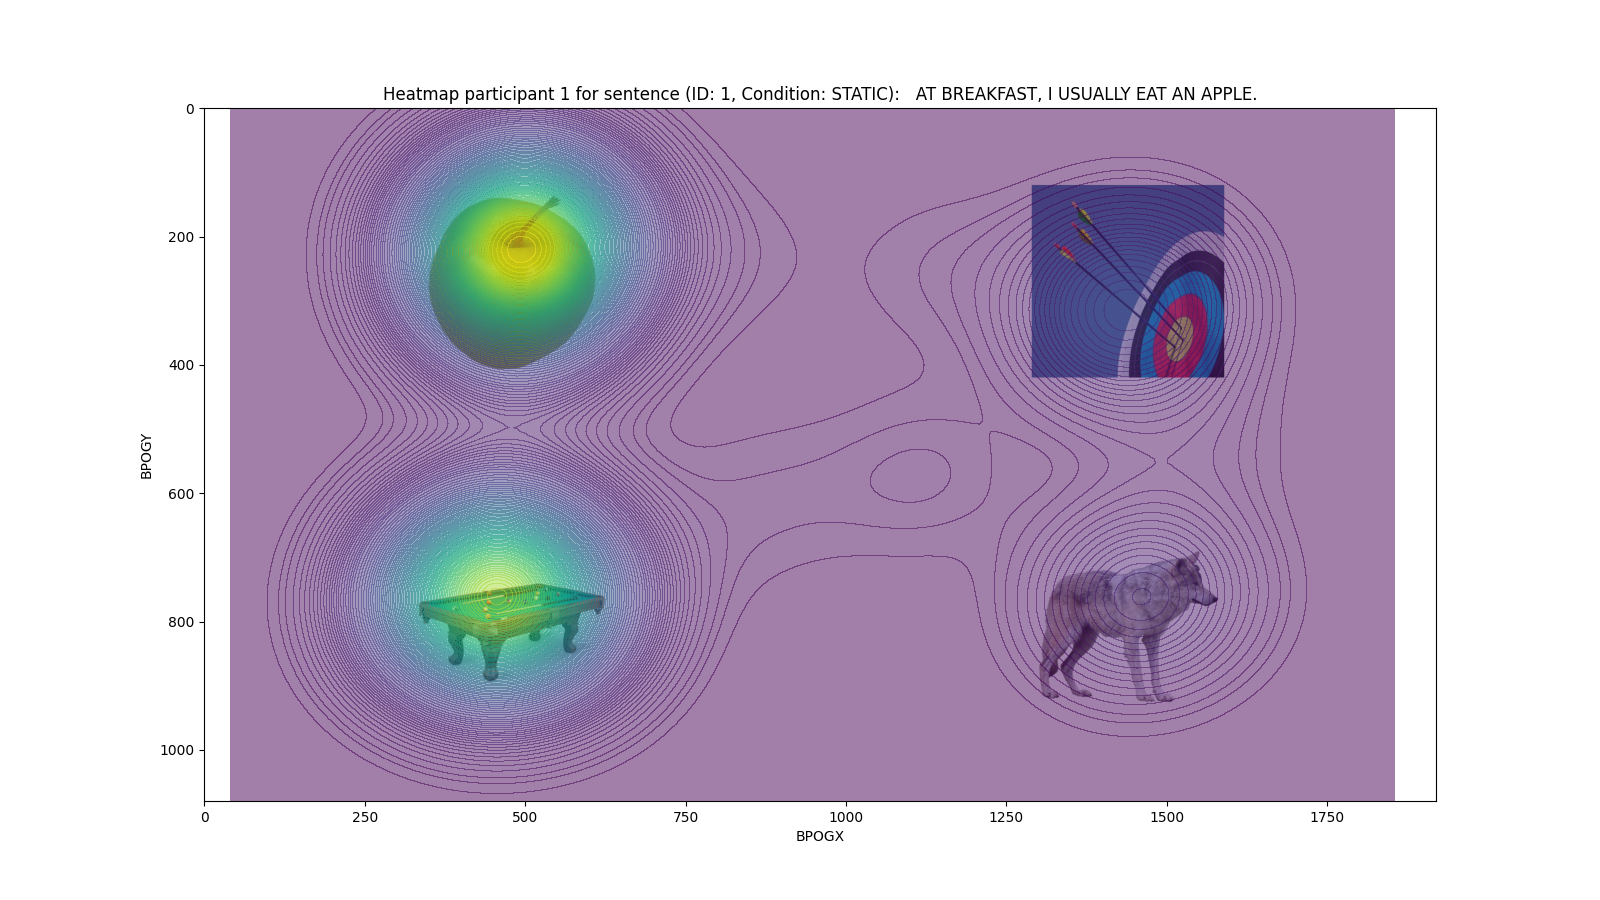
\includegraphics{Images/Fig4_4_2.png}

}

\caption{\label{fig-heatmap}Example heatmap for a sentence}

\end{figure}%

To determine whether a participant directed their gaze toward a target,
two primary types of eye movements can be looked at: fixations and
saccades.

When considering saccades, several variations of this metric might be
interesting to see if the anticipation effect persist when adding motion
stimuli. An example therefore would be the first saccade after the
target word of a sentence is said. However, the inclusion of such a
metric requires precise experimental timing and raises several
methodological questions. For example, how should saccades that initiate
immediately after the target cue be handled? Overall, saccades are not
sufficiently robust for this analysis and introduce a lot of noise,
making them impractical within the scope of this project.

Conversely, fixations provide a more straightforward metric. In this
study, we are not interested in the duration of fixations or the precise
location of the gaze point. Instead, the primary focus is on determining
whether the participant is looking at a specific target. Given this
requirement, we chose not to analyze fixations directly. Instead, we
opted to use the samples from the eye tracker. These samples are more
robust and less noisy since they do not need to undergo a fixation
detection algorithm, which can create additional noise.

Given the need to accurately detect the specific sub-stimulus at which a
participant is looking, four areas of interest were defined. These AOIs
correspond to the locations of each sub-stimulus and are slightly larger
(350 pixels) than the resolution of each sub-stimulus (300 pixels). This
setup results in four AOIs: top-left (TL), top-right (TR), bottom-left
(BL), and bottom-right (BR). The center of each AOI corresponds to the
relative position of each sub-stimulus to the middle. For example the
center top-left AOI is 1/4 of the width and 1/4 of the height. An
algorithm was implemented that considers the center positions and
calculate two intervals where the BPOGX and BPOGY of a sample need to be
located in order to be considered inside the bounding box (see
Listing~\ref{lst-alg-aoi}). Since our metrics base on the AOIs, the
algorithm was tested with additional visualisations (see
Figure~\ref{fig-aoi-valid}) and could be used in the further course of
the analysis.

\begin{codelisting}

\caption{\label{lst-alg-aoi}}

\centering{

\begin{Shaded}
\begin{Highlighting}[]
\CommentTok{\# function that checks wheather subject looked at desired area of interest}
\KeywordTok{def}\NormalTok{ bpog\_in\_target\_bbox(bpogx, bpogy, pos):}

    \CommentTok{\# var "width" and "height" are globally (static) definded}

\NormalTok{    x }\OperatorTok{=}\NormalTok{ bpogx }\OperatorTok{*}\NormalTok{ width}
\NormalTok{    y }\OperatorTok{=}\NormalTok{ bpogy }\OperatorTok{*}\NormalTok{ height}
    
    \ControlFlowTok{if}\NormalTok{ pos }\OperatorTok{==} \StringTok{"TL"}\NormalTok{:}
\NormalTok{        relpos }\OperatorTok{=}\NormalTok{ (width}\OperatorTok{/}\DecValTok{4}\NormalTok{, height}\OperatorTok{/}\DecValTok{4}\NormalTok{)}
    \ControlFlowTok{elif}\NormalTok{ pos }\OperatorTok{==} \StringTok{"TR"}\NormalTok{:}
\NormalTok{        relpos }\OperatorTok{=}\NormalTok{ (width}\OperatorTok{*}\NormalTok{(}\DecValTok{3}\OperatorTok{/}\DecValTok{4}\NormalTok{), height}\OperatorTok{/}\DecValTok{4}\NormalTok{)}
    \ControlFlowTok{elif}\NormalTok{ pos }\OperatorTok{==} \StringTok{"BL"}\NormalTok{:}
\NormalTok{        relpos }\OperatorTok{=}\NormalTok{ (width}\OperatorTok{/}\DecValTok{4}\NormalTok{, height}\OperatorTok{*}\NormalTok{(}\DecValTok{3}\OperatorTok{/}\DecValTok{4}\NormalTok{))}
    \ControlFlowTok{elif}\NormalTok{ pos }\OperatorTok{==} \StringTok{"BR"}\NormalTok{:}
\NormalTok{        relpos }\OperatorTok{=}\NormalTok{ (width}\OperatorTok{*}\NormalTok{(}\DecValTok{3}\OperatorTok{/}\DecValTok{4}\NormalTok{), height}\OperatorTok{*}\NormalTok{(}\DecValTok{3}\OperatorTok{/}\DecValTok{4}\NormalTok{))}
    \ControlFlowTok{else}\NormalTok{:}
\NormalTok{        relpos }\OperatorTok{=} \OperatorTok{{-}}\DecValTok{1}

    \CommentTok{\# add/rest 150 + 50 to relative position }
\NormalTok{    pos\_x\_l }\OperatorTok{=}\NormalTok{ relpos[}\DecValTok{0}\NormalTok{] }\OperatorTok{{-}} \DecValTok{200}
\NormalTok{    pos\_x\_r }\OperatorTok{=}\NormalTok{ relpos[}\DecValTok{0}\NormalTok{] }\OperatorTok{+} \DecValTok{200}
\NormalTok{    pos\_y\_d }\OperatorTok{=}\NormalTok{ relpos[}\DecValTok{1}\NormalTok{] }\OperatorTok{{-}} \DecValTok{200}
\NormalTok{    pos\_y\_u }\OperatorTok{=}\NormalTok{ relpos[}\DecValTok{1}\NormalTok{] }\OperatorTok{+} \DecValTok{200}

    \CommentTok{\# check if in area of interest box}
    \ControlFlowTok{if}\NormalTok{ (x }\OperatorTok{\textgreater{}}\NormalTok{ pos\_x\_l) }\KeywordTok{and}\NormalTok{ (x }\OperatorTok{\textless{}}\NormalTok{ pos\_x\_r):}
        \ControlFlowTok{if}\NormalTok{(y }\OperatorTok{\textgreater{}}\NormalTok{ pos\_y\_d) }\KeywordTok{and}\NormalTok{ (y }\OperatorTok{\textless{}}\NormalTok{ pos\_y\_u):}
            \ControlFlowTok{return} \VariableTok{True}

    \ControlFlowTok{return} \VariableTok{False}
\end{Highlighting}
\end{Shaded}

}

\end{codelisting}%

\begin{figure}

\centering{

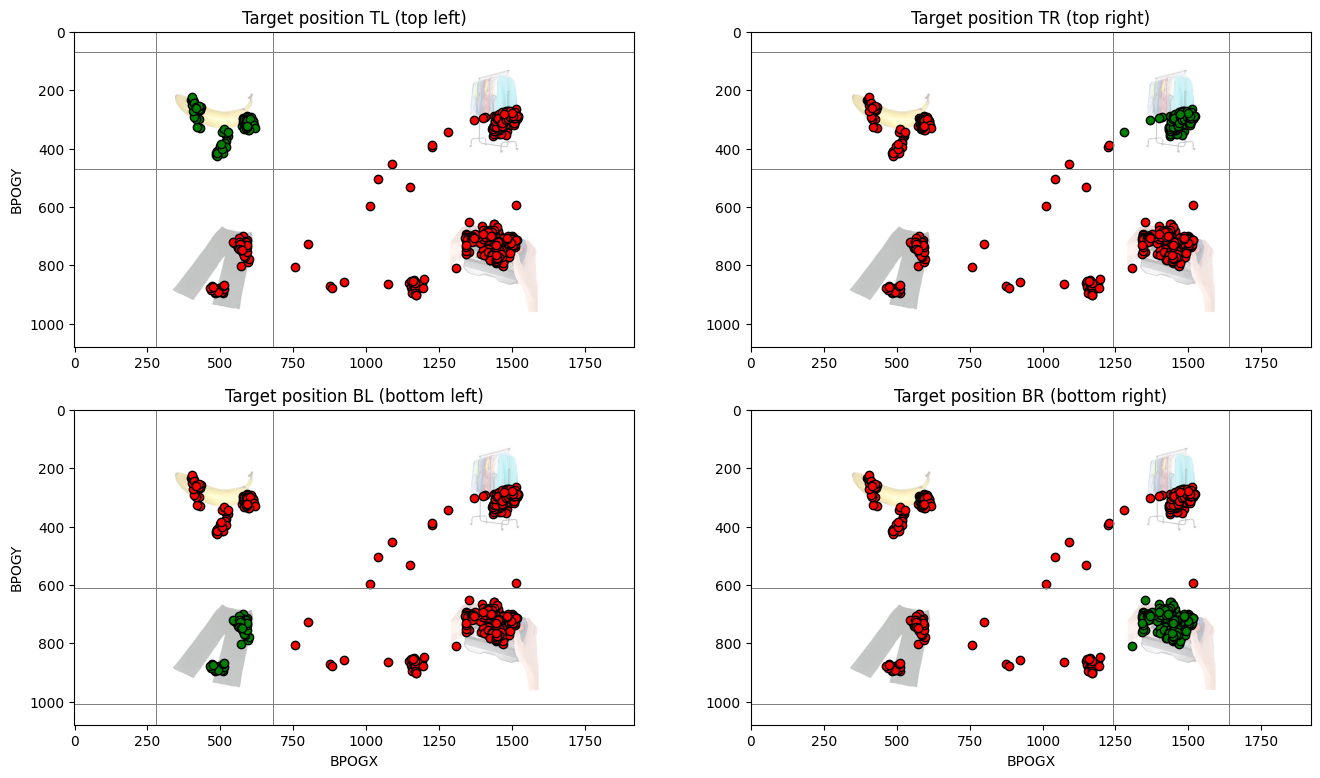
\includegraphics{Images/Fig4_4_10.png}

}

\caption{\label{fig-aoi-valid}Area of interest verification algorithm}

\end{figure}%

With the area of interest fixation algorthmen, we can now have a look at
the two metrics of this experiment. The target ratio and the non-target
ratio. The target ratio describes the samples that were detected inside
the target area of interest in relation to the total amount of examples.
The non-target ratio describes the samples that were detected in all
other areas of interest except the target aoi in relation to the total
samples.

\[
TR = \frac{\text{Samples on target AOI}}{\text{Total samples}}
\] \[
NTR = \frac{\text{Samples on non-target AOIs}}{\text{Total samples}}
\]

With this two introduced metrics, a variety of interesting analysis and
visualisations is possible. The target and non-target ratio can be
looked at for an individual subject and sentence with a specific
condition (see Figure~\ref{fig-trntrstatic}).

\begin{figure}

\centering{

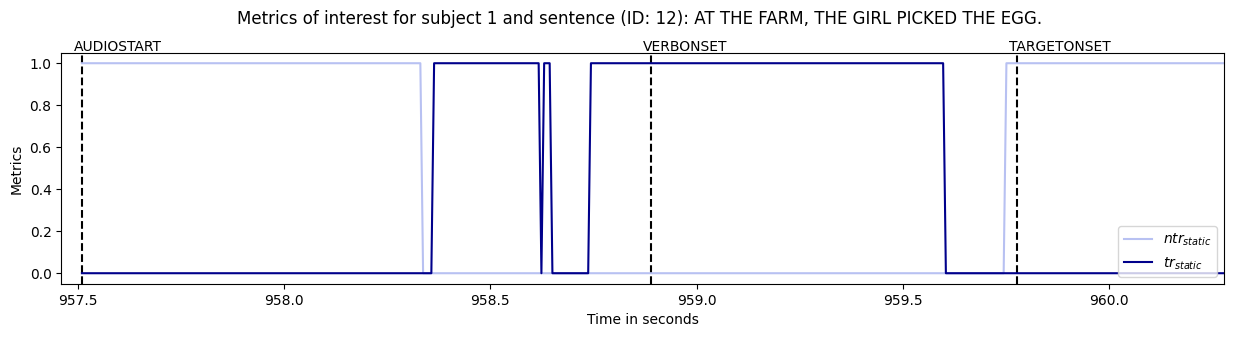
\includegraphics{Images/Fig4_4_9.png}

}

\caption{\label{fig-trntrstatic}Example targt ratio and non-target ratio
for the static condition}

\end{figure}%

Another interesting insight is the average tr and ntr over all subjects
for one sentence (see Figure~\ref{fig-trntrsentence}).

\begin{figure}

\centering{

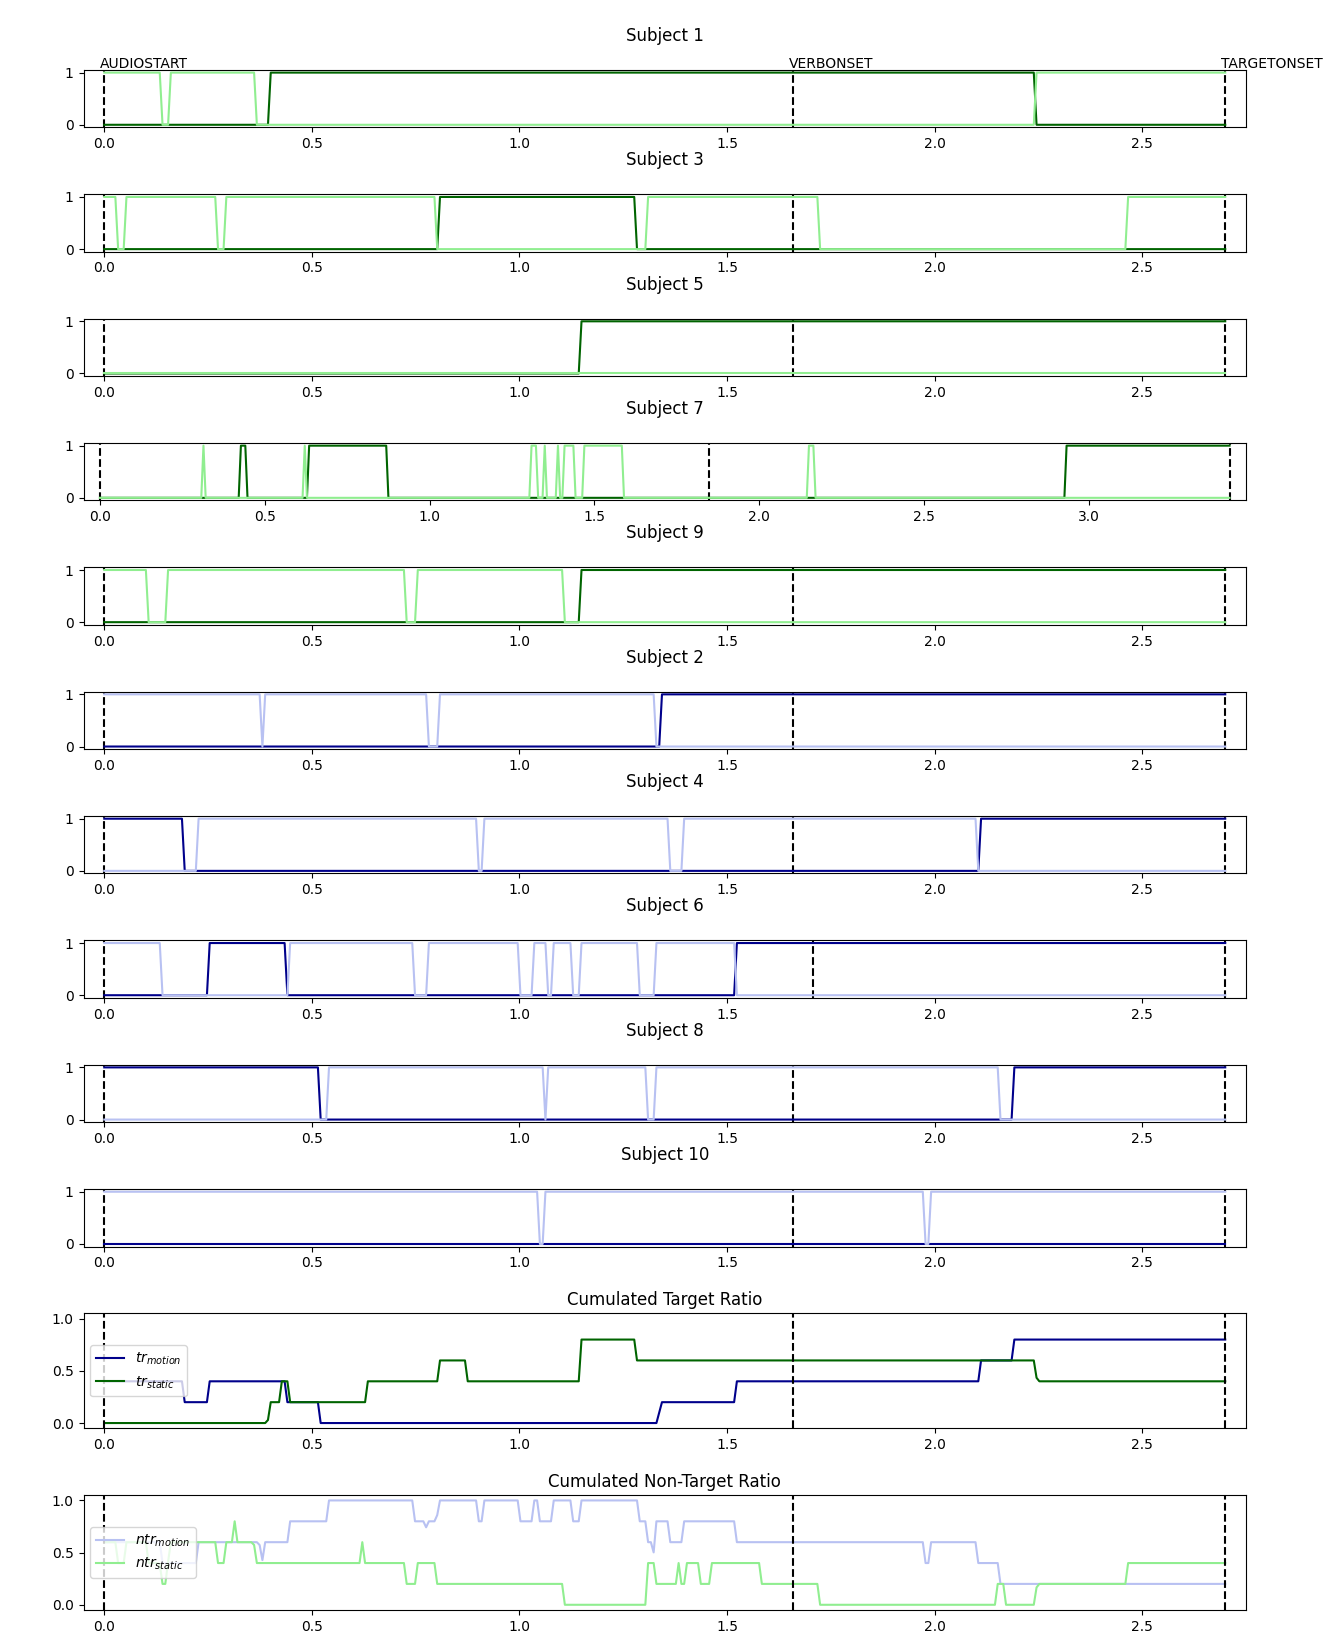
\includegraphics{Images/Fig4_4_8.png}

}

\caption{\label{fig-trntrsentence}Example TR and NTR for an example
sentence over all subjects}

\end{figure}%

Our goal is to compare the target ratio and non-target ratio for
sentences with the static condition to the sentences with the motion
condition. The TR and NTR are measured exactly 50 miliseconds before the
\emph{TARGETONSET} event and thereby before the target word is said.
Since its only one measure point the TR and NTR for a single sentence
can be 1 or 0. For each subject the average target and non-target ratio
for all sentences with the static condition \emph{tr(static)} and motion
condition \emph{tr(motion)} is calculated.

With the resulting metrics for each subjects, the total average, mean
and standard deviation is calculated, visualized in a boxplot and
interpreted.

The scripts to calculate all metrics mentioned above can be found in the
project folder under \emph{\textasciitilde/scripts/}.

\chapter{Results}\label{sec-results}

In the following we present the results of our conducted experiment. We
collected mainly quantitative data by recording the gaze of our
participants, but we extended it with qualitative data by keeping lab
notes for each participant to have more context for salient gaze
behavior.

\section{Participants}\label{participants}

We had 10 people participating in our experiment between the ages 18 and
34 where nine people identified as male and one as female. Regarding
their English level, most (6) people specified that they have reached at
least a C1 level and the remaining (4) people were at a B2 level.
Additionally, we asked the participants about their previous experience
with eye-tracking. For the majority (7) it was the first time using
eye-trackers, the other three stated that they have used eye-trackers
before.

Overall, all the participants were able to complete the experiment
successfully without significant complications.

\section{Pilot Data}\label{pilot-data}

The initial data visualizations with the pilot data gave us a first
impression of the data we were about to collect and provided us a
semantic santiy check, whether our experiment design is actually
suitable for the research question we had in mind. The visualizations
additionally gave us valuable feedback on the technical implementation
of the experiment. Through the visualization we decided to remove the
fixation dot in the middle of the screen when the stimuli are visible,
since it inadverently directed the participant's gaze to some extend.

\begin{figure}

\centering{

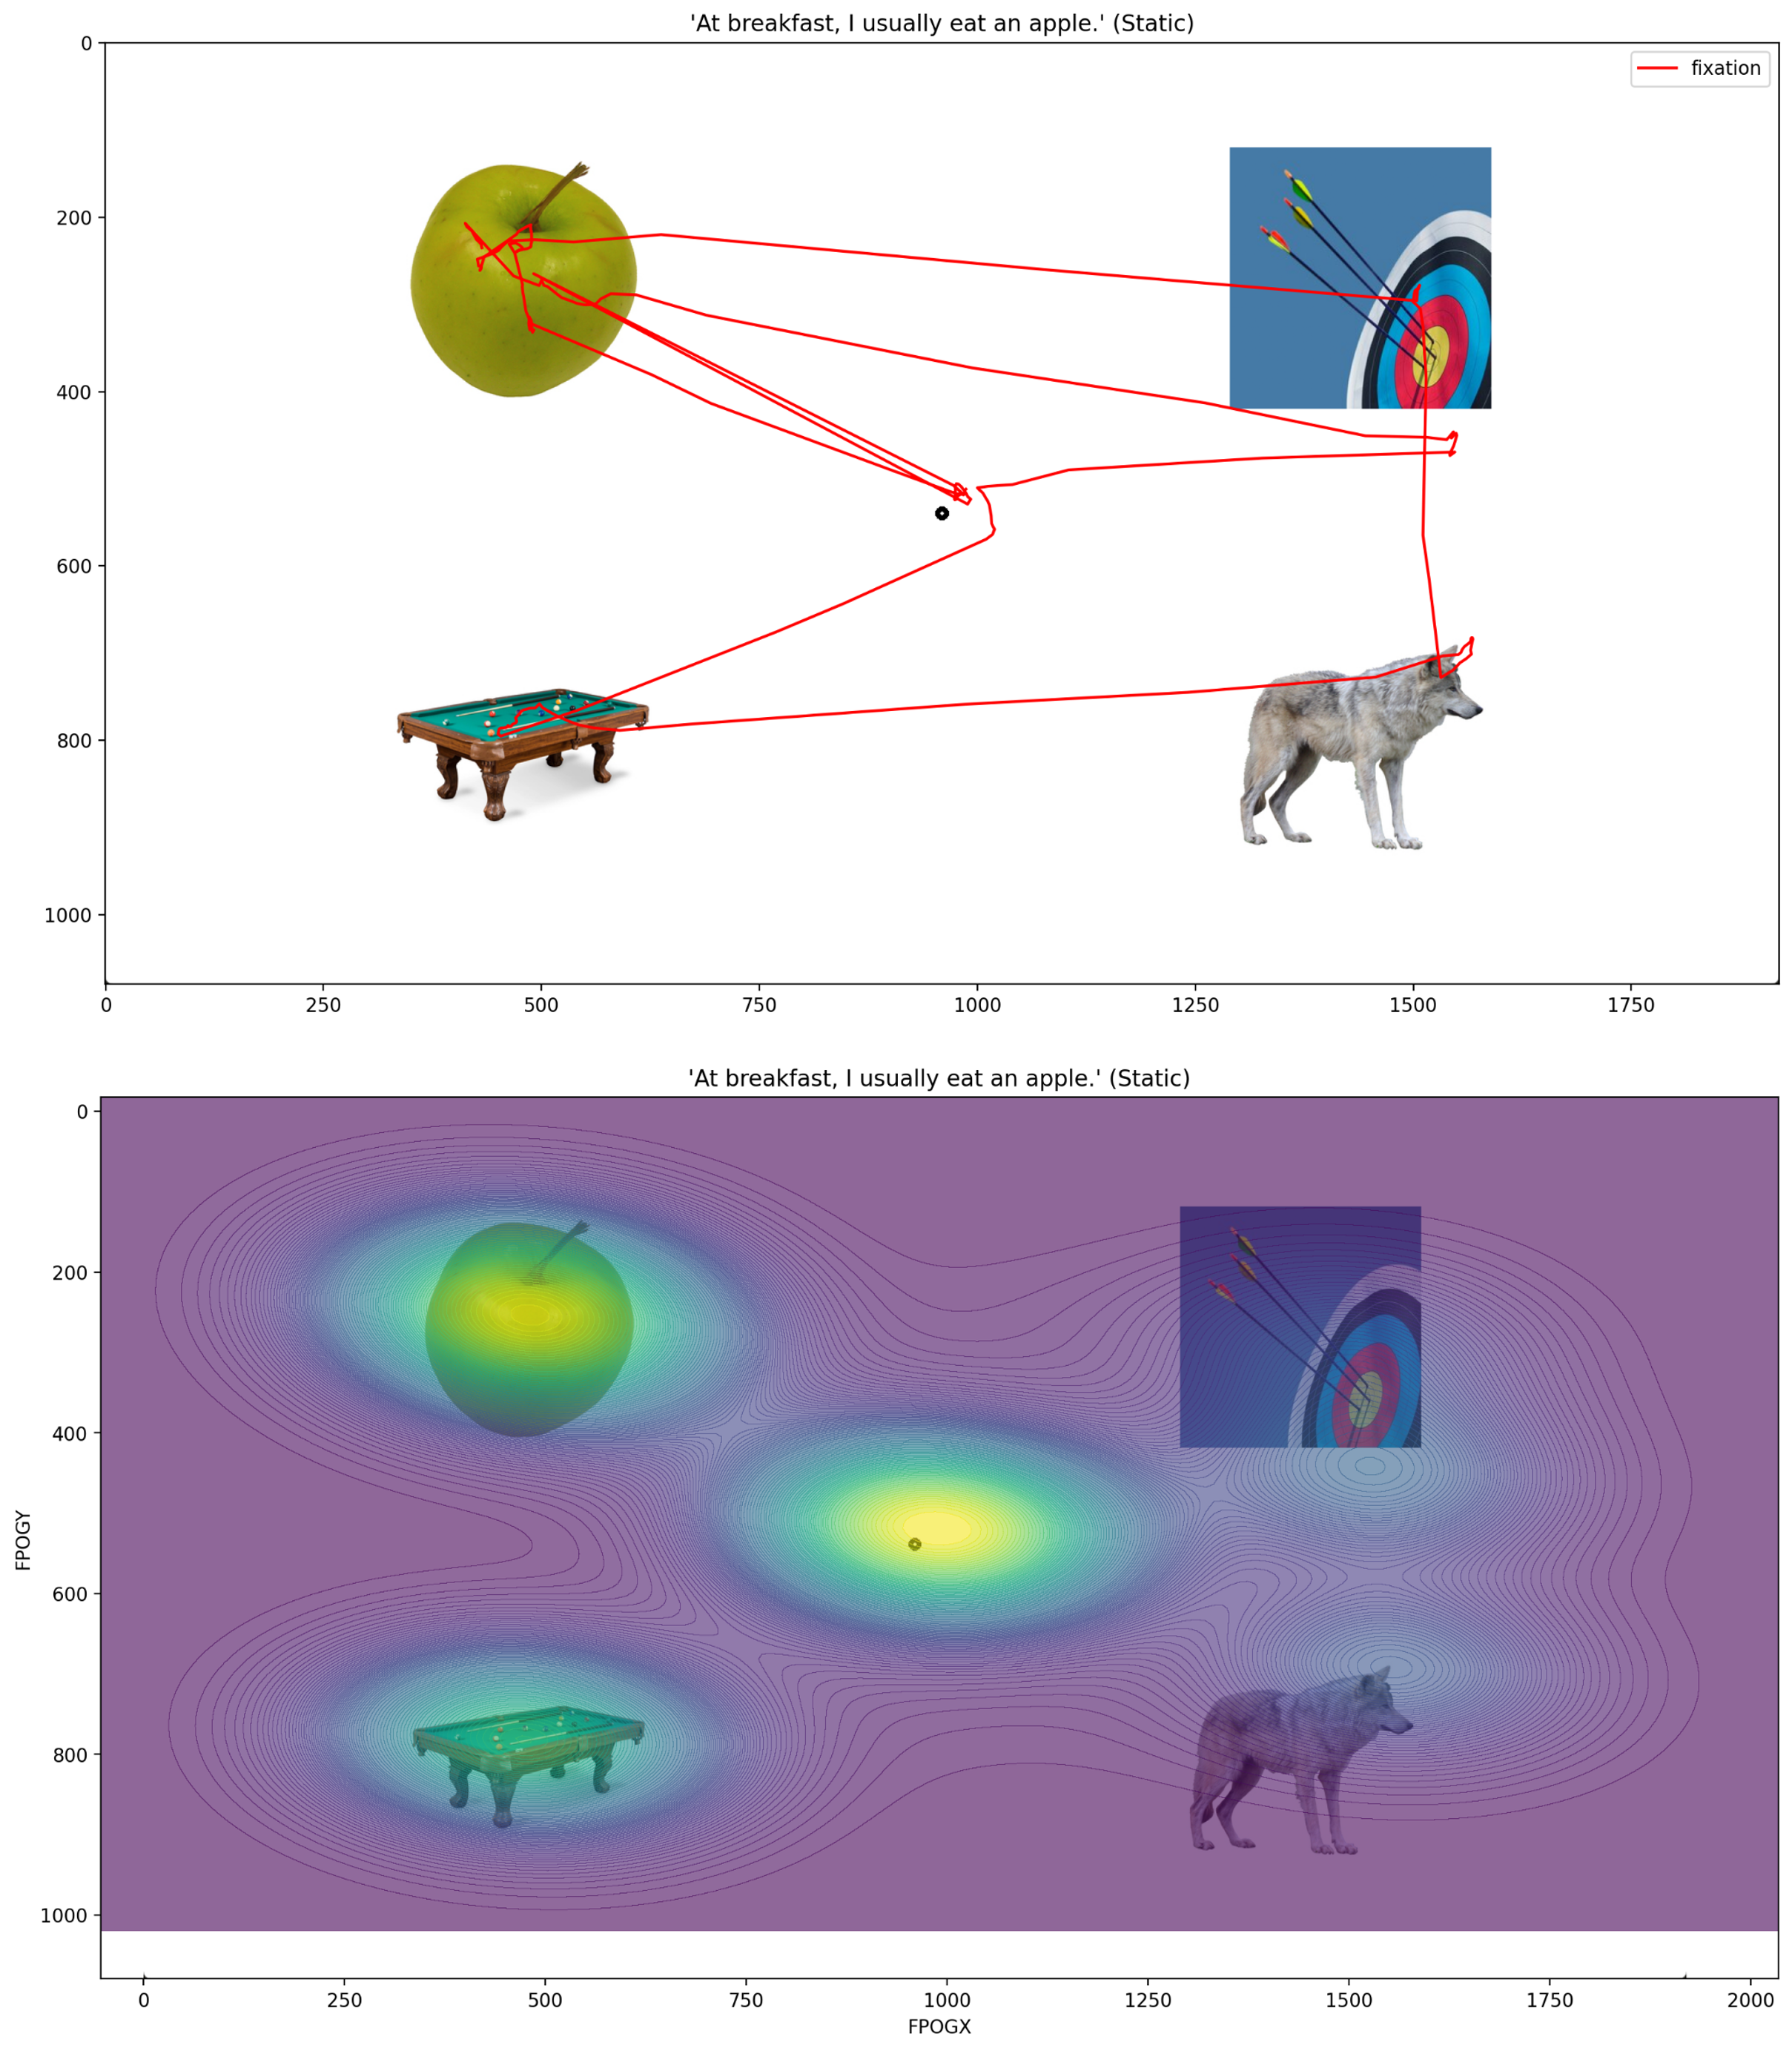
\includegraphics{Images/Fig9_8_7.png}

}

\caption{\label{fig-pilot}Visualized pilot data including sub-stimuli
with fixdot}

\end{figure}%

\section{Gaze on Target Behavior}\label{gaze-on-target-behavior}

Figure~\ref{fig-boxplot-global} illustrates the boxplots for the mean TR
and NTR as well as the static and motion conditions for all
participants. Overall the interquartile range (IQR) of TR for the motion
condition is slightly higher than for the static. The static condition
is shifted by around 0.2 towards higher values. Althought the TR-median
is 0.1 higher for the motion condition. The values of NTR behave in an
opposite way. This indicates that the IQR is higher for the static
condition and shifted by 0.2 towards lower values. The NTR share for
both conditions the same median. Additionally, metrics that are not
directly visible in the boxplot, as well as supplementary metrics, can
be found in Table~\ref{tbl-condition-group-comparison}. The values from
the table emphasize the insights from the boxplot and demonstrate that
the TR is marginally higher for the static condition than the motion
condition.

\begin{figure}

\centering{

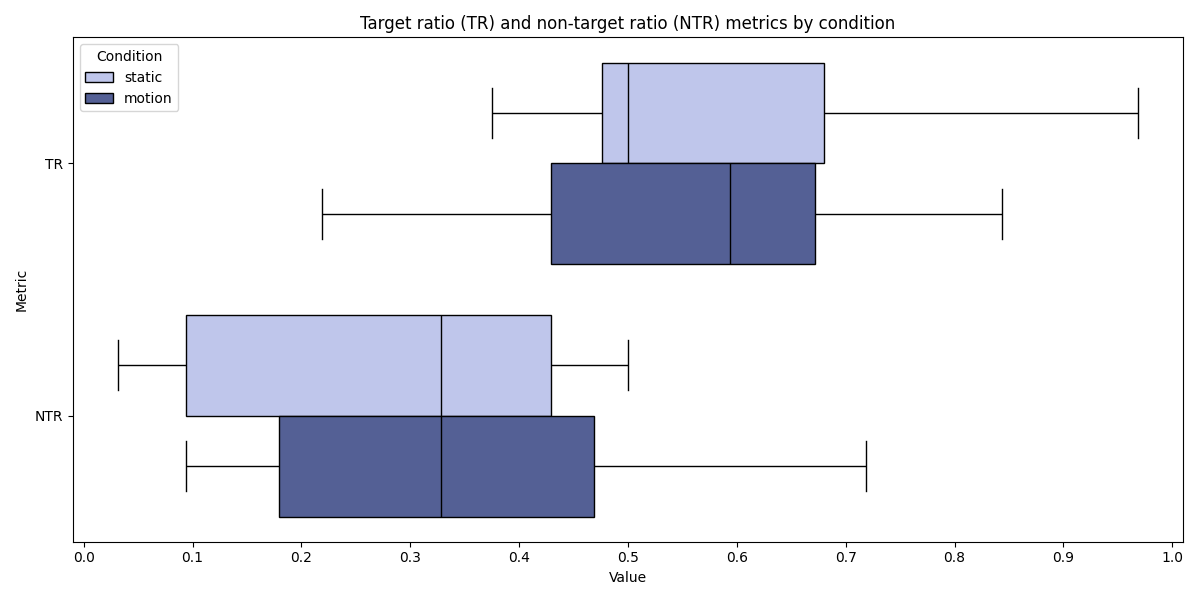
\includegraphics{Images/4-analysis-boxplot-tr-and-ntr.png}

}

\caption{\label{fig-boxplot-global}Boxplot diagrams of our main metrics
for both static and motion conditions}

\end{figure}%

\begin{longtable}[]{@{}lccc@{}}
\caption{Metric comparison between the participant groups and the
complete data set
(global)}\label{tbl-condition-group-comparison}\tabularnewline
\toprule\noalign{}
Metric & Global & Wolf & Chicken \\
\midrule\noalign{}
\endfirsthead
\toprule\noalign{}
Metric & Global & Wolf & Chicken \\
\midrule\noalign{}
\endhead
\bottomrule\noalign{}
\endlastfoot
Mean TR (static) & 0.594 & 0.625 & 0.562 \\
Mean TR (motion) & 0.559 & 0.6 & 0.519 \\
Mean NTR (static) & 0.275 & 0.194 & 0.356 \\
Mean NTR (motion) & 0.353 & 0.275 & 0.431 \\
Stdev TR (static) & 0.367 & 0.492 & 0.225 \\
Stdev TR (motion) & 0.273 & 0.374 & 0.185 \\
Stdev NTR (static) & 0.174 & 0.187 & 0.111 \\
Stdev NTR (motion) & 0.197 & 0.194 & 0.166 \\
\end{longtable}

Furthermore, we split the analysis up to our two participant groups to
check, if we obtain noticeable differences in the data. The data is
listed in Table~\ref{tbl-condition-group-comparison} and visualized as
boxplots in Figure~\ref{fig-boxplot-chicken} and
Figure~\ref{fig-boxplot-wolf}.

\begin{figure}

\centering{

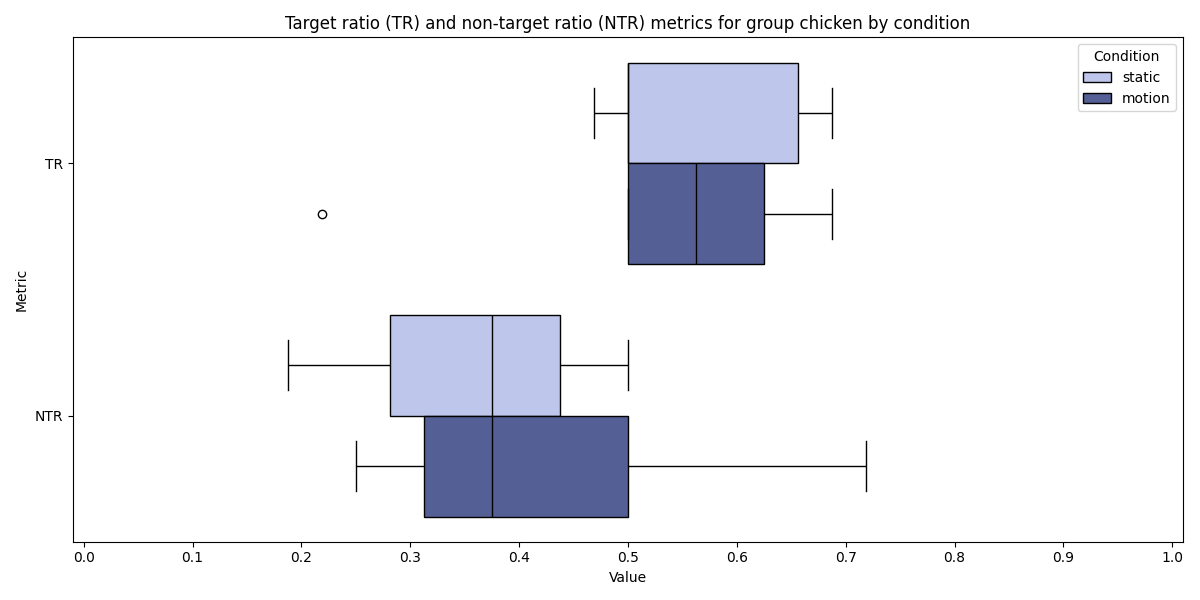
\includegraphics{Images/4-analysis-boxplot-chicken-tr-and-ntr.png}

}

\caption{\label{fig-boxplot-chicken}Boxplot diagrams of our main metrics
for both static and motion conditions for the participant group chicken}

\end{figure}%

\begin{figure}

\centering{

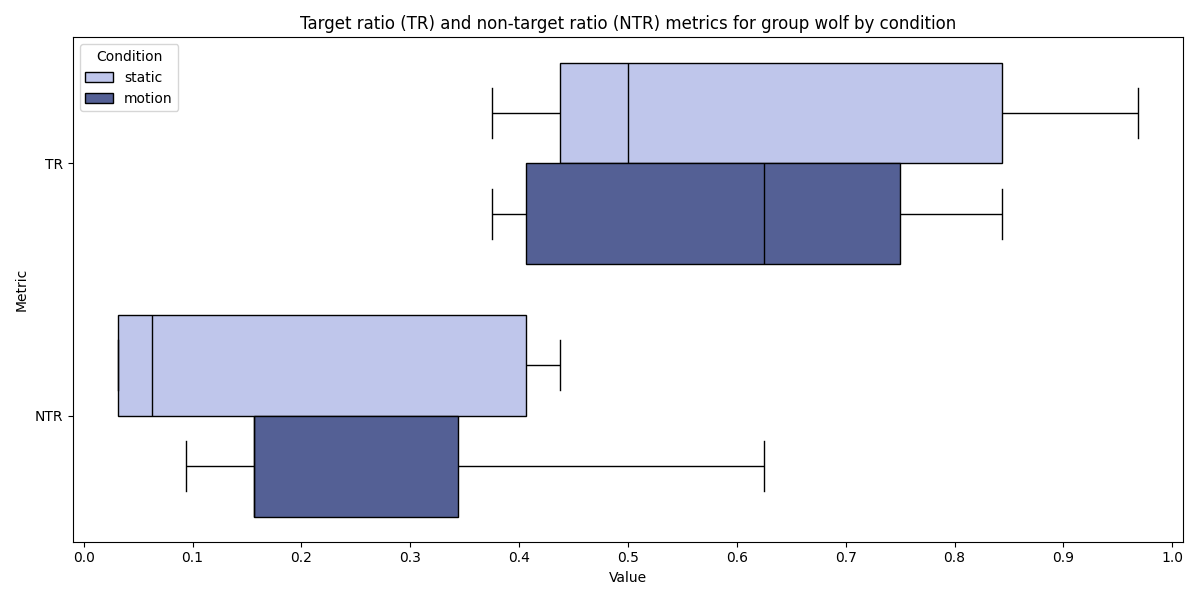
\includegraphics{Images/4-analysis-boxplot-wolf-tr-and-ntr.png}

}

\caption{\label{fig-boxplot-wolf}Boxplot diagrams of our main metrics
for both static and motion conditions group wolf}

\end{figure}%

The results indicate, that there is a larger standard deviation in the
static condition in group wolf compared to group chicken. However, we
can still identify the same trend that we saw in the global analysis,
which is that the static conditon performs slightly better (higher
target rate) than the motion condtion. Another thing to note here is
that we only have five participants in each group, meaning that these
statistical analyses are more sensitive to outliers.

\chapter{Discussion}\label{sec-discussion}

Discussion

1- paragraph Summary

How do the findings relate to the literature?

Limitations

Challenges during project

Our results show that our participants did look at related objects in
the visual stimuli before hearing it in a sentence, by infering from
previous parts of the sentence, such as the verb or the real-world
context they appear in. This anticipation effect was more visible in the
static condition data, which was set up similarly to previous work by
Gerry T. M. Altmann and Kamide (1999). The second motion condition,
altough showing lower results compared to the static one, indicate that
the participants still made anticipatory eye movements before hearing
the target word at the end of the sentence. The added movement in the
stimuli might be a distracting factor which lowered the anticipation
effect, but due to our small effect size, we cannot claim this
assumption with high confidence. Another limiting factor to our study is
unlike the previously referenced work, we did not conduct the study with
native speakers of the English language. Altering the stimuli to be in
German would introduce a series of new questions we would need to ask
ourselves regarding the stimuli design, and due to the limited scope of
this course, we decided to keep the study design as simple as possible
and orientied it by our previously referenced work.

Adding to our list of limitations, we did not collect much qualitative
data in our study. Including open-ended questions in our questionnaire
at the end might have helped to put the gaze data of our participants
more into context and potentially collect feedback on the experiment
design overall.

We observed some of our participants getting bored during the
experiment, either they told us or they started fidgeting more during
the trials seeming impatient. This indicates that we should plan a short
break halfway through the trials, since the participants might not feel
the need to speak up about needing a short break.

\section{Outlook/ improvements / Lessons
learned}\label{outlook-improvements-lessons-learned}

In conclusion, we\ldots{}

What we have learned during this project\ldots{} - how challenging
stimuli design is -

In the following, we propose related key topics to be adressed in the
future: \ldots{} - Conduct the experiment in more ``lab-like''
conditions e.g.~more uniform stimuli, having native speakers of the
language used in the study as participants, overall more participants to
obtain more robust results

\begin{itemize}
\item
  do people still make predicting eye movements when target is static
  and distractors are moving?
\item
  how about when target is moving and distractors are static? How to mix
  these conditions?
\end{itemize}

\chapter{Contribution Table}\label{contribution-table}

The following table gives a detailed insight on how the workload of this
project was split between the group members:

\begin{longtable}[]{@{}llll@{}}
\toprule\noalign{}
Task & Yanhong & Dilara & Karl Jorge \\
\midrule\noalign{}
\endhead
\bottomrule\noalign{}
\endlastfoot
Background Literature & x & o & \\
Experiment Design & & x & \\
Experiment Implementation & & & x \\
Stimulus and audio design & x & & \\
Piloting & & x & x \\
Pilot plots & & & x \\
Data-Recording & o & x & x \\
Data Analysis Scripts & & & x \\
Report Writing & o & x & o \\
Report Lectorate & x & & \\
Participant Acquisition & x & x & x \\
Project Management & & x & \\
\end{longtable}

Legend: x = main, o = supporter

\phantomsection\label{refs}
\begin{CSLReferences}{1}{0}
\bibitem[\citeproctext]{ref-abrams_motion_2003}
Abrams, Richard A., and Shawn E. Christ. 2003. {``Motion {Onset}
{Captures} {Attention}.''} \emph{Psychol Sci} 14 (5): 427--32.
\url{https://doi.org/10.1111/1467-9280.01458}.

\bibitem[\citeproctext]{ref-altmann_thematic_1999}
Altmann, Gerry T. M. 1999. {``Thematic {Role} {Assignment} in
{Context}.''} \emph{Journal of Memory and Language} 41 (1): 124--45.
\url{https://doi.org/10.1006/jmla.1999.2640}.

\bibitem[\citeproctext]{ref-altmann_incremental_1999}
Altmann, Gerry T. M, and Yuki Kamide. 1999. {``Incremental
Interpretation at Verbs: Restricting the Domain of Subsequent
Reference.''} \emph{Cognition} 73 (3): 247--64.
\url{https://doi.org/10.1016/S0010-0277(99)00059-1}.

\bibitem[\citeproctext]{ref-schmid_eye-tracking_2016}
Berends, Sanne M., Susanne M. Brouwer, and Simone A. Sprenger. 2016.
{``Eye-{Tracking} and the {Visual} {World} {Paradigm}.''} In
\emph{Designing {Research} on {Bilingual} {Development}}, 55--80. Cham:
Springer International Publishing.
\url{https://doi.org/10.1007/978-3-319-11529-0_5}.

\bibitem[\citeproctext]{ref-cooper_control_1974}
Cooper, Roger M. 1974. {``The Control of Eye Fixation by the Meaning of
Spoken Language: {A} New Methodology for the Real-Time Investigation of
Speech Perception, Memory, and Language Processing.''} \emph{Cognitive
Psychology} 6 (1): 84--107.
\url{https://doi.org/10.1016/0010-0285(74)90005-X}.

\bibitem[\citeproctext]{ref-elgort_cross-language_2023}
Elgort, Irina, Marc Brysbaert, and Anna Siyanova-Chanturia. 2023.
{``Cross-Language {Influences} in {Bilingual} {Processing} and {Second}
{Language} {Acquisition},''} 1--327.
\url{https://doi.org/10.1075/bpa.16}.

\bibitem[\citeproctext]{ref-huettig_using_2011}
Huettig, Falk, Joost Rommers, and Antje S. Meyer. 2011. {``Using the
Visual World Paradigm to Study Language Processing: {A} Review and
Critical Evaluation.''} \emph{Acta Psychologica}, Visual search and
visual world: {Interactions} among visual attention, language, and
working memory, 137 (2): 151--71.
\url{https://doi.org/10.1016/j.actpsy.2010.11.003}.

\bibitem[\citeproctext]{ref-spencer2016stereotype}
Spencer, Steven J, Christine Logel, and Paul G Davies. 2016.
{``Stereotype Threat.''} \emph{Annual Review of Psychology} 67: 415--37.
\url{https://doi.org/10.1111/j.1559-1816.2008.00362.x}.

\bibitem[\citeproctext]{ref-tanenhaus_integration_1995}
Tanenhaus, Michael K., Michael J. Spivey-Knowlton, Kathleen M. Eberhard,
and Julie C. Sedivy. 1995. {``Integration of {Visual} and {Linguistic}
{Information} in {Spoken} {Language} {Comprehension}.''} \emph{Science}
268 (5217): 1632--34. \url{https://doi.org/10.1126/science.7777863}.

\end{CSLReferences}




\end{document}
